
\section{Horizontal Droplet View}

\par This experiment served as an initiation to the camera use. As stated before, the geometric implications of the droplet shape in radiation prevent the extraction of quantitative results.\\
\par This experiment was made in two different speeds: 2 m/s and 0.8 m/s, and three temperatures: 60ºC, 100ºC and 110ºC. A sample of the results of this experiment can be seen in Figure \ref{fig:hexp}. In this figure, the x axis represents the distance between the bottom of the droplet to its top. These results show that within the same speed, the temperature gradient evolves similarly between different temperatures, along the time. It is also noticeable the high temperature in the interface and the considerably lower temperature at the top.

\begin{figure}[h]
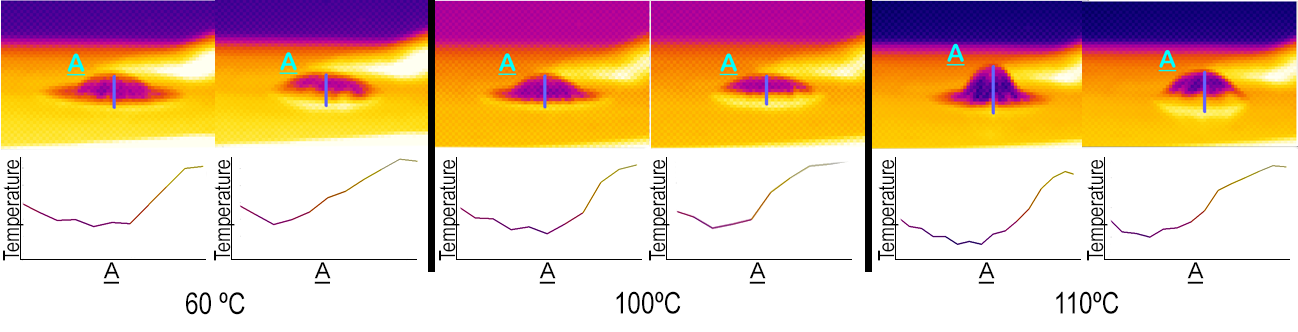
\includegraphics[width=1\linewidth]{Figures/5.Chapter/hexp.png}
\caption{Horizontal Results for 2 m/s during the spreading and receding phases}
\label{fig:hexp}
\end{figure}

\section{Bottom View}

\par The shown results will have a similar structure. Reading through this section, it is important to bear in mind that the results shown for a certain experiment can have both a bidimensional temperature map and a plot with temperatures along the radius for certain time-frames. The relation between the temperature maps, plots and the real image can be seen in Figure 

\begin{figure}[h]
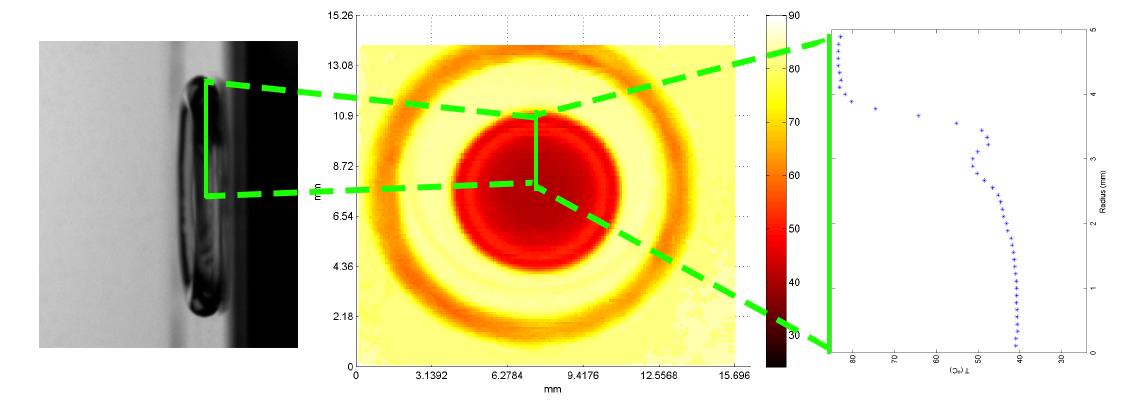
\includegraphics[width=1\linewidth]{Figures/5.Chapter/example.png}
\caption{Example of the results representation}
\label{fig:hexp}
\end{figure}

\par In the Bottom View experimental setup, various conditions were tested. Two different impact velocity values, with different characteristics: 0.8 m/s and 2 m/s. Four initial foil temperature values, representing conditions before and after saturation: 60ºC, 80ºC, 100ºC and 110ºC. Two different wettability, hydrophilic and hydrophobic, surfaces were tested. Finally, tests were also made with two liquids: water and ethanol. For each of the conditions, 5 different experiments were made, so that the repeatability of the tests could be confirmed. In Figure \ref{fig:repeat} the repeatability of these tests can be seen with the example of the 60ºC results for 2 m/s.\\

\begin{figure}
\centering
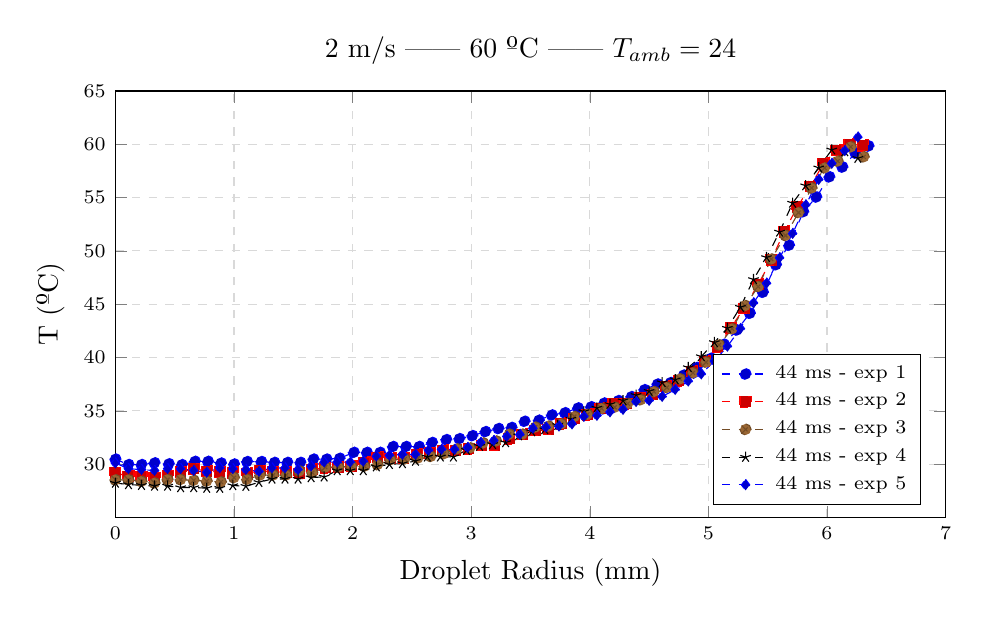
\begin{tikzpicture}
\begin{axis}[
	title = {2 m/s || 60 ºC || $T_{amb}=24$},
    tick label style={font=\scriptsize},
    legend style={font=\scriptsize,/tikz/column 2/.style={column sep=5pt},},
    %legend columns=2,
    legend cell align=left,
	legend pos =south east,
    grid=major, % Display a grid
    grid style={dashed,gray!30}, % Set the style
    xlabel={Droplet Radius (mm)},
    ylabel={T (ºC)}, 
    ymin = 25, ymax = 65,
    ytick={30,35,...,120},
    %yticklabels={300,325,350,375,400,425,450,475,500,525},
    xmin = 0, xmax = 7,
    %ytick={0,1600,...,11200},
    %yticklabel style={
    %    /pgf/number format/fixed,
    %    /pgf/number format/precision=5},
	%scaled y ticks=false,
    width=1\textwidth, 
    height=7cm,
    cycle list name= color
    ]
\addplot+[dashed]
coordinates {(	0	,	30.48	)
(	0.11	,	29.97	)
(	0.22	,	29.97	)
(	0.33	,	30.13	)
(	0.45	,	30.04	)
(	0.56	,	29.96	)
(	0.67	,	30.27	)
(	0.78	,	30.27	)
(	0.89	,	30.11	)
(	1	,	30.02	)
(	1.11	,	30.25	)
(	1.23	,	30.25	)
(	1.34	,	30.17	)
(	1.45	,	30.17	)
(	1.56	,	30.17	)
(	1.67	,	30.48	)
(	1.78	,	30.48	)
(	1.89	,	30.56	)
(	2.01	,	31.11	)
(	2.12	,	31.11	)
(	2.23	,	31.11	)
(	2.34	,	31.66	)
(	2.45	,	31.66	)
(	2.56	,	31.66	)
(	2.67	,	32.04	)
(	2.79	,	32.31	)
(	2.9	,	32.4	)
(	3.01	,	32.68	)
(	3.12	,	33.06	)
(	3.23	,	33.35	)
(	3.34	,	33.45	)
(	3.45	,	34.03	)
(	3.57	,	34.13	)
(	3.68	,	34.62	)
(	3.79	,	34.83	)
(	3.9	,	35.28	)
(	4.01	,	35.39	)
(	4.12	,	35.74	)
(	4.24	,	35.97	)
(	4.35	,	36.34	)
(	4.46	,	36.99	)
(	4.57	,	37.52	)
(	4.68	,	37.66	)
(	4.79	,	38.36	)
(	4.9	,	39.07	)
(	5.02	,	39.94	)
(	5.13	,	41.25	)
(	5.24	,	42.58	)
(	5.35	,	44.15	)
(	5.46	,	46.12	)
(	5.57	,	48.7	)
(	5.68	,	50.53	)
(	5.8	,	53.67	)
(	5.91	,	55.05	)
(	6.02	,	56.94	)
(	6.13	,	57.86	)
(	6.24	,	59.17	)
(	6.35	,	59.83	)
};
\addlegendentry{44 ms - exp 1}

\addplot+[dashed]
coordinates {(	0	,	29.18	)
(	0.11	,	28.88	)
(	0.22	,	28.81	)
(	0.33	,	28.73	)
(	0.44	,	28.9	)
(	0.55	,	29.28	)
(	0.66	,	29.58	)
(	0.77	,	29.36	)
(	0.88	,	29.29	)
(	0.99	,	29.22	)
(	1.11	,	29.15	)
(	1.22	,	29.38	)
(	1.33	,	29.31	)
(	1.44	,	29.24	)
(	1.55	,	29.17	)
(	1.66	,	29.53	)
(	1.77	,	29.66	)
(	1.88	,	29.73	)
(	1.99	,	29.8	)
(	2.1	,	30.16	)
(	2.21	,	30.66	)
(	2.32	,	30.58	)
(	2.43	,	30.58	)
(	2.54	,	30.93	)
(	2.65	,	31.08	)
(	2.76	,	31.31	)
(	2.87	,	31.31	)
(	2.98	,	31.47	)
(	3.09	,	31.78	)
(	3.2	,	31.78	)
(	3.32	,	32.39	)
(	3.43	,	32.83	)
(	3.54	,	33.18	)
(	3.65	,	33.27	)
(	3.76	,	33.82	)
(	3.87	,	34.28	)
(	3.98	,	34.67	)
(	4.09	,	35.24	)
(	4.2	,	35.67	)
(	4.31	,	35.67	)
(	4.42	,	36.22	)
(	4.53	,	36.57	)
(	4.64	,	37.31	)
(	4.75	,	37.81	)
(	4.86	,	38.72	)
(	4.97	,	39.67	)
(	5.08	,	41.03	)
(	5.19	,	42.81	)
(	5.3	,	44.63	)
(	5.42	,	46.87	)
(	5.53	,	49.15	)
(	5.64	,	51.83	)
(	5.75	,	54.13	)
(	5.86	,	56.06	)
(	5.97	,	58.19	)
(	6.08	,	59.43	)
(	6.19	,	60.02	)
(	6.3	,	59.89	)
};
\addlegendentry{44 ms - exp 2}

\addplot+[dashed]
coordinates {(	0	,	28.54	)
(	0.11	,	28.54	)
(	0.22	,	28.39	)
(	0.33	,	28.24	)
(	0.44	,	28.56	)
(	0.55	,	28.56	)
(	0.66	,	28.49	)
(	0.77	,	28.42	)
(	0.89	,	28.34	)
(	1	,	28.74	)
(	1.11	,	28.59	)
(	1.22	,	28.98	)
(	1.33	,	28.98	)
(	1.44	,	28.98	)
(	1.55	,	29.36	)
(	1.66	,	29.21	)
(	1.77	,	29.73	)
(	1.88	,	29.73	)
(	1.99	,	29.81	)
(	2.1	,	29.81	)
(	2.21	,	29.96	)
(	2.32	,	30.41	)
(	2.44	,	30.49	)
(	2.55	,	30.57	)
(	2.66	,	30.73	)
(	2.77	,	30.98	)
(	2.88	,	31.44	)
(	2.99	,	31.53	)
(	3.1	,	31.99	)
(	3.21	,	32.17	)
(	3.32	,	32.82	)
(	3.43	,	32.82	)
(	3.54	,	33.48	)
(	3.65	,	33.58	)
(	3.76	,	33.78	)
(	3.87	,	34.47	)
(	3.98	,	34.68	)
(	4.1	,	35.23	)
(	4.21	,	35.34	)
(	4.32	,	35.69	)
(	4.43	,	36.04	)
(	4.54	,	36.81	)
(	4.65	,	37.2	)
(	4.76	,	38	)
(	4.87	,	38.57	)
(	4.98	,	39.57	)
(	5.09	,	41.19	)
(	5.2	,	42.7	)
(	5.31	,	44.87	)
(	5.42	,	46.66	)
(	5.53	,	49.24	)
(	5.65	,	51.45	)
(	5.76	,	53.6	)
(	5.87	,	55.9	)
(	5.98	,	57.78	)
(	6.09	,	58.42	)
(	6.2	,	59.75	)
(	6.31	,	58.82	)
};
\addlegendentry{44 ms - exp 3}

\addplot+[dashed]
coordinates {(	0	,	28.24	)
(	0.11	,	28.1	)
(	0.22	,	28.03	)
(	0.33	,	27.96	)
(	0.44	,	27.96	)
(	0.55	,	27.82	)
(	0.66	,	27.82	)
(	0.77	,	27.76	)
(	0.88	,	27.76	)
(	0.99	,	28.01	)
(	1.1	,	27.94	)
(	1.21	,	28.31	)
(	1.32	,	28.62	)
(	1.43	,	28.62	)
(	1.54	,	28.62	)
(	1.65	,	28.75	)
(	1.76	,	28.82	)
(	1.87	,	29.41	)
(	1.98	,	29.41	)
(	2.09	,	29.41	)
(	2.2	,	29.77	)
(	2.31	,	29.99	)
(	2.42	,	30.07	)
(	2.53	,	30.3	)
(	2.63	,	30.69	)
(	2.74	,	30.69	)
(	2.85	,	30.69	)
(	2.96	,	31.32	)
(	3.07	,	31.69	)
(	3.18	,	31.86	)
(	3.29	,	32.04	)
(	3.4	,	32.68	)
(	3.51	,	33.06	)
(	3.62	,	33.25	)
(	3.73	,	33.65	)
(	3.84	,	34.24	)
(	3.95	,	34.94	)
(	4.06	,	35.28	)
(	4.17	,	35.62	)
(	4.28	,	35.97	)
(	4.39	,	36.47	)
(	4.5	,	36.85	)
(	4.61	,	37.66	)
(	4.72	,	37.93	)
(	4.83	,	39.07	)
(	4.94	,	40.1	)
(	5.05	,	41.42	)
(	5.16	,	42.76	)
(	5.27	,	44.73	)
(	5.38	,	47.33	)
(	5.49	,	49.39	)
(	5.6	,	51.78	)
(	5.71	,	54.49	)
(	5.82	,	56.12	)
(	5.93	,	57.8	)
(	6.04	,	59.48	)
(	6.15	,	59.31	)
(	6.26	,	58.69	)
};
\addlegendentry{44 ms - exp 4}

\addplot+[dashed]
coordinates {(	0	,	30.11	)
(	0.11	,	29.58	)
(	0.22	,	29.5	)
(	0.33	,	29.41	)
(	0.44	,	29.58	)
(	0.55	,	29.58	)
(	0.66	,	29.41	)
(	0.77	,	29.24	)
(	0.88	,	29.66	)
(	0.99	,	29.57	)
(	1.1	,	29.49	)
(	1.21	,	29.33	)
(	1.32	,	29.65	)
(	1.43	,	29.65	)
(	1.54	,	29.49	)
(	1.65	,	29.81	)
(	1.76	,	30.2	)
(	1.87	,	30.2	)
(	1.98	,	30.2	)
(	2.09	,	30.28	)
(	2.2	,	30.75	)
(	2.31	,	30.84	)
(	2.42	,	30.92	)
(	2.53	,	30.92	)
(	2.64	,	31.31	)
(	2.75	,	31.39	)
(	2.86	,	31.39	)
(	2.97	,	31.57	)
(	3.08	,	32.04	)
(	3.19	,	32.22	)
(	3.3	,	32.61	)
(	3.41	,	32.79	)
(	3.52	,	33.37	)
(	3.63	,	33.47	)
(	3.74	,	33.57	)
(	3.85	,	33.77	)
(	3.95	,	34.47	)
(	4.06	,	34.57	)
(	4.17	,	34.9	)
(	4.28	,	35.13	)
(	4.39	,	35.87	)
(	4.5	,	35.98	)
(	4.61	,	36.35	)
(	4.72	,	37	)
(	4.83	,	37.79	)
(	4.94	,	38.46	)
(	5.05	,	39.67	)
(	5.16	,	41.06	)
(	5.27	,	42.71	)
(	5.38	,	45.12	)
(	5.49	,	46.97	)
(	5.6	,	49.35	)
(	5.71	,	51.63	)
(	5.82	,	54.3	)
(	5.93	,	56.69	)
(	6.04	,	58.2	)
(	6.15	,	59.39	)
(	6.26	,	60.66	)
};
\addlegendentry{44 ms - exp 5}
\end{axis}
\end{tikzpicture}
\caption{Repeatability of the experiments}
\label{fig:repeat}
\end{figure}

\subsection{Before the Calibration}

\par Before the calibration method was used, some preliminary results were taken for comparison. To evaluate the quality of the calibration it is important to compare the results and interpret the differences. The same results were taken from the experiments before the calibration, than after the calibration. For the speeds of 2 m/s and 0.8 m/s, the foil temperatures of 60ºC, 100ºC and 110ºC were analyzed. A sample taken of the results before and after the applied method can be seen in Figure \ref{fig:calibcomp2}. \\

\par Before comparing the images, one should bare in mind the differences in their conditions. The results before calibration were taken at a different ambient temperature, and framerate. The average framerate of the results before the calibration is 990 fps, and 1100 after. One can only compare similar frames and differences may be accentuated by that. \\
\par One important aspect is that the diameter is approximately the same, which means that the droplets we can see, during the spreading phase (all the points before 23 ms) the new calibration and method captures a bit of the air trapping effect mentioned previously in Section \ref{sec:heat}, while this effect is not present in the results without the calibration. Another thing that was corrected, was the fact that the temperature would drop bellow the ambient temperature before the calibration. This is impossible because the droplet is at ambient temperature. The cause of this happening has roots on optical effects, that were nullified by the calibration. On the other side the calibrated camera results have some noise that couldn't be addressed without losing resolution. The cause of the noise is probably the improved installation that allowed for higher spatial resolution. So while there is advantages in the factory calibration, the proposed calibration can better portrait the physical phenomena. \\

\begin{figure}
\centering
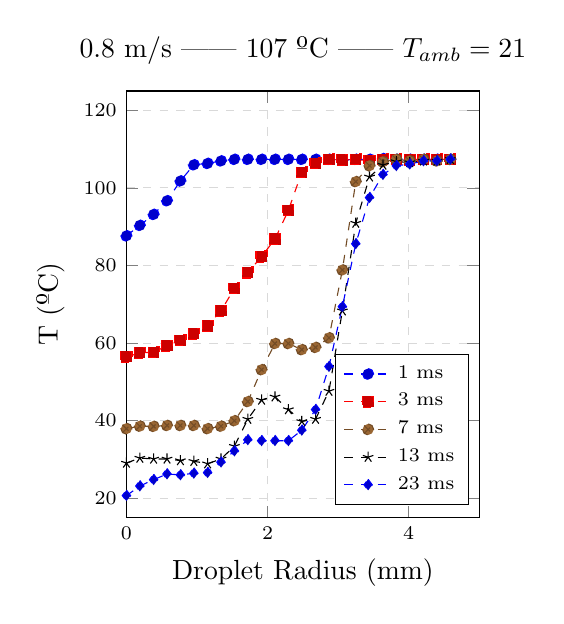
\begin{tikzpicture}
\begin{axis}[
	title = {0.8 m/s || 107 ºC || $T_{amb}=21$},
    tick label style={font=\scriptsize},
    legend style={font=\scriptsize,/tikz/column 2/.style={column sep=5pt},},
    %legend columns=2,
    legend cell align=left,
	legend pos =south east,
    grid=major, % Display a grid
    grid style={dashed,gray!30}, % Set the style
    xlabel={Droplet Radius (mm)},
    ylabel={T (ºC)}, 
    ymin = 15, ymax = 125,
    ytick={20,40,...,120},
    %yticklabels={300,325,350,375,400,425,450,475,500,525},
    xmin = 0, xmax = 5,
    %ytick={0,1600,...,11200},
    %yticklabel style={
    %    /pgf/number format/fixed,
    %    /pgf/number format/precision=5},
	%scaled y ticks=false,
    width=0.5\textwidth, 
    height=7cm,
    cycle list name= color
    ]
\addplot+[dashed]
coordinates {(	0	,	87.65	)
(	0.19	,	90.34	)
(	0.385	,	93.17	)
(	0.575	,	96.69	)
(	0.765	,	101.8	)
(	0.955	,	105.96	)
(	1.15	,	106.32	)
(	1.34	,	106.96	)
(	1.53	,	107.37	)
(	1.72	,	107.37	)
(	1.915	,	107.37	)
(	2.105	,	107.37	)
(	2.295	,	107.37	)
(	2.485	,	107.37	)
(	2.68	,	107.37	)
(	2.87	,	107.37	)
(	3.06	,	107.19	)
(	3.25	,	107.37	)
(	3.445	,	107.37	)
(	3.635	,	107.55	)
(	3.825	,	107.37	)
(	4.015	,	107.37	)
(	4.21	,	107.37	)
(	4.4	,	107.37	)
(	4.59	,	107.37	)
};
\addlegendentry{1 ms}

\addplot+[dashed]
coordinates {(	0	,	56.42	)
(	0.19	,	57.47	)
(	0.385	,	57.65	)
(	0.575	,	59.29	)
(	0.765	,	60.71	)
(	0.955	,	62.4	)
(	1.15	,	64.4	)
(	1.34	,	68.33	)
(	1.53	,	74.09	)
(	1.72	,	78.19	)
(	1.915	,	82.3	)
(	2.105	,	86.82	)
(	2.295	,	94.22	)
(	2.485	,	104.08	)
(	2.68	,	106.32	)
(	2.87	,	107.37	)
(	3.06	,	107.19	)
(	3.25	,	107.37	)
(	3.445	,	106.96	)
(	3.635	,	107.37	)
(	3.825	,	107.37	)
(	4.015	,	107.19	)
(	4.21	,	107.37	)
(	4.4	,	107.37	)
(	4.59	,	107.37	)
};
\addlegendentry{3 ms}

\addplot+[dashed]
coordinates {(	0	,	37.93	)
(	0.19	,	38.57	)
(	0.385	,	38.52	)
(	0.575	,	38.75	)
(	0.765	,	38.75	)
(	0.955	,	38.75	)
(	1.15	,	37.93	)
(	1.34	,	38.57	)
(	1.53	,	39.98	)
(	1.72	,	44.91	)
(	1.915	,	53.13	)
(	2.105	,	59.88	)
(	2.295	,	59.88	)
(	2.485	,	58.29	)
(	2.68	,	58.88	)
(	2.87	,	61.35	)
(	3.06	,	78.84	)
(	3.25	,	101.62	)
(	3.445	,	105.72	)
(	3.635	,	106.73	)
(	3.825	,	107.37	)
(	4.015	,	106.96	)
(	4.21	,	107.37	)
(	4.4	,	106.96	)
(	4.59	,	107.37	)
};
\addlegendentry{7 ms}

\addplot+[dashed]
coordinates {(	0	,	29.07	)
(	0.19	,	30.35	)
(	0.385	,	30.12	)
(	0.575	,	30.12	)
(	0.765	,	29.71	)
(	0.955	,	29.53	)
(	1.15	,	28.89	)
(	1.34	,	30.12	)
(	1.53	,	33.41	)
(	1.72	,	40.39	)
(	1.915	,	45.32	)
(	2.105	,	46.14	)
(	2.295	,	42.86	)
(	2.485	,	39.8	)
(	2.68	,	40.39	)
(	2.87	,	47.61	)
(	3.06	,	68.33	)
(	3.25	,	90.93	)
(	3.445	,	102.85	)
(	3.635	,	105.9	)
(	3.825	,	106.78	)
(	4.015	,	106.55	)
(	4.21	,	106.96	)
(	4.4	,	106.96	)
(	4.59	,	107.37	)
};
\addlegendentry{13 ms}

\addplot+[dashed]
coordinates {(	0	,	20.67	)
(	0.19	,	23.13	)
(	0.385	,	24.78	)
(	0.575	,	26.24	)
(	0.765	,	26.01	)
(	0.955	,	26.42	)
(	1.15	,	26.6	)
(	1.34	,	29.3	)
(	1.53	,	32.17	)
(	1.72	,	35.05	)
(	1.915	,	34.82	)
(	2.105	,	34.82	)
(	2.295	,	34.82	)
(	2.485	,	37.52	)
(	2.68	,	42.86	)
(	2.87	,	53.95	)
(	3.06	,	69.39	)
(	3.25	,	85.59	)
(	3.445	,	97.51	)
(	3.635	,	103.44	)
(	3.825	,	105.72	)
(	4.015	,	106.14	)
(	4.21	,	106.96	)
(	4.4	,	106.96	)
(	4.59	,	107.37	)
};
\addlegendentry{23 ms}
\end{axis}
\end{tikzpicture}
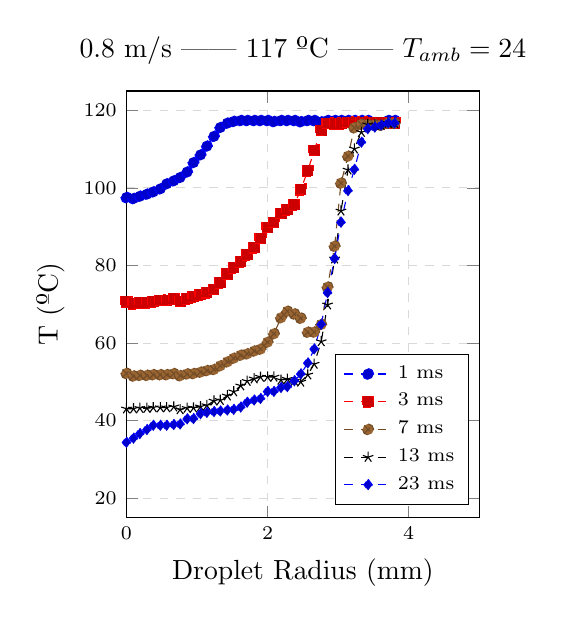
\begin{tikzpicture}
\begin{axis}[
	title = {0.8 m/s || 117 ºC || $T_{amb}=24$},
    tick label style={font=\scriptsize},
    legend style={font=\scriptsize,/tikz/column 2/.style={column sep=5pt},},
    %legend columns=2,
    legend cell align=left,
	legend pos =south east,
    grid=major, % Display a grid
    grid style={dashed,gray!30}, % Set the style
    xlabel={Droplet Radius (mm)},
    ylabel={T (ºC)}, 
    ymin = 15, ymax = 125,
    ytick={20,40,...,120},
    %yticklabels={300,325,350,375,400,425,450,475,500,525},
    xmin = 0, xmax = 5,
    %ytick={0,1600,...,11200},
    %yticklabel style={
    %    /pgf/number format/fixed,
    %    /pgf/number format/precision=5},
	%scaled y ticks=false,
    width=0.5\textwidth, height=7cm,
    cycle list name= color
    ]
\addplot+[dashed]
coordinates {(	0	,	97.52	)
(	0.1	,	97.26	)
(	0.19	,	97.85	)
(	0.29	,	98.38	)
(	0.38	,	98.98	)
(	0.48	,	99.76	)
(	0.57	,	101.05	)
(	0.67	,	101.82	)
(	0.76	,	102.68	)
(	0.86	,	104.1	)
(	0.95	,	106.53	)
(	1.05	,	108.52	)
(	1.14	,	110.77	)
(	1.24	,	113.29	)
(	1.33	,	115.57	)
(	1.43	,	116.69	)
(	1.52	,	117.14	)
(	1.62	,	117.37	)
(	1.71	,	117.37	)
(	1.81	,	117.37	)
(	1.9	,	117.37	)
(	2	,	117.37	)
(	2.09	,	117.1	)
(	2.19	,	117.37	)
(	2.28	,	117.37	)
(	2.38	,	117.37	)
(	2.47	,	117.06	)
(	2.57	,	117.37	)
(	2.66	,	117.37	)
(	2.76	,	117.02	)
(	2.85	,	117.37	)
(	2.95	,	117.37	)
(	3.04	,	117.37	)
(	3.14	,	117.37	)
(	3.23	,	117.37	)
(	3.33	,	117.37	)
(	3.42	,	117.37	)
(	3.52	,	116.8	)
(	3.61	,	116.76	)
(	3.71	,	117.37	)
(	3.8	,	117.37	)
};
\addlegendentry{1 ms}

\addplot+[dashed]
coordinates {(	0	,	70.61	)
(	0.1	,	70.16	)
(	0.19	,	70.4	)
(	0.29	,	70.4	)
(	0.38	,	70.63	)
(	0.48	,	71.08	)
(	0.57	,	71.08	)
(	0.67	,	71.45	)
(	0.76	,	70.78	)
(	0.86	,	71.41	)
(	0.95	,	71.99	)
(	1.05	,	72.51	)
(	1.14	,	73.05	)
(	1.24	,	73.92	)
(	1.33	,	75.58	)
(	1.43	,	77.81	)
(	1.52	,	79.42	)
(	1.62	,	80.97	)
(	1.71	,	82.76	)
(	1.81	,	84.66	)
(	1.9	,	87.07	)
(	2	,	89.89	)
(	2.09	,	91.11	)
(	2.19	,	93.47	)
(	2.28	,	94.33	)
(	2.38	,	95.68	)
(	2.47	,	99.61	)
(	2.57	,	104.39	)
(	2.66	,	109.67	)
(	2.76	,	114.9	)
(	2.85	,	116.64	)
(	2.95	,	116.6	)
(	3.04	,	116.54	)
(	3.14	,	116.94	)
(	3.23	,	116.91	)
(	3.33	,	116.88	)
(	3.42	,	116.84	)
(	3.52	,	116.8	)
(	3.61	,	116.76	)
(	3.71	,	116.7	)
(	3.8	,	116.65	)
};
\addlegendentry{3 ms}

\addplot+[dashed]
coordinates {(	0	,	52.18	)
(	0.1	,	51.5	)
(	0.19	,	51.67	)
(	0.29	,	51.67	)
(	0.38	,	51.84	)
(	0.48	,	51.84	)
(	0.57	,	51.84	)
(	0.67	,	52.11	)
(	0.76	,	51.58	)
(	0.86	,	52.04	)
(	0.95	,	52.13	)
(	1.05	,	52.5	)
(	1.14	,	52.89	)
(	1.24	,	53.19	)
(	1.33	,	54.12	)
(	1.43	,	55.15	)
(	1.52	,	56.08	)
(	1.62	,	56.86	)
(	1.71	,	57.21	)
(	1.81	,	57.93	)
(	1.9	,	58.43	)
(	2	,	60.23	)
(	2.09	,	62.39	)
(	2.19	,	66.52	)
(	2.28	,	68.19	)
(	2.38	,	67.5	)
(	2.47	,	66.4	)
(	2.57	,	62.8	)
(	2.66	,	62.84	)
(	2.76	,	64.79	)
(	2.85	,	74.42	)
(	2.95	,	84.98	)
(	3.04	,	101.24	)
(	3.14	,	108.17	)
(	3.23	,	115.5	)
(	3.33	,	116.38	)
(	3.42	,	116.3	)
(	3.52	,	116.22	)
(	3.61	,	116.14	)
(	3.71	,	116.7	)
(	3.8	,	116.65	)
};
\addlegendentry{7 ms}

\addplot+[dashed]
coordinates {(	0	,	43.06	)
(	0.1	,	43.06	)
(	0.19	,	43.2	)
(	0.29	,	43.2	)
(	0.38	,	43.35	)
(	0.48	,	43.35	)
(	0.57	,	43.35	)
(	0.67	,	43.57	)
(	0.76	,	42.84	)
(	0.86	,	43.21	)
(	0.95	,	43.29	)
(	1.05	,	43.6	)
(	1.14	,	43.92	)
(	1.24	,	45.08	)
(	1.33	,	45.25	)
(	1.43	,	46.41	)
(	1.52	,	47.47	)
(	1.62	,	49	)
(	1.71	,	50.17	)
(	1.81	,	50.8	)
(	1.9	,	51.24	)
(	2	,	51.26	)
(	2.09	,	51.26	)
(	2.19	,	50.46	)
(	2.28	,	50.71	)
(	2.38	,	50.22	)
(	2.47	,	49.97	)
(	2.57	,	51.82	)
(	2.66	,	54.59	)
(	2.76	,	60.39	)
(	2.85	,	69.88	)
(	2.95	,	81.73	)
(	3.04	,	94.08	)
(	3.14	,	104.64	)
(	3.23	,	110.08	)
(	3.33	,	114.35	)
(	3.42	,	116.3	)
(	3.52	,	116.22	)
(	3.61	,	116.14	)
(	3.71	,	116.7	)
(	3.8	,	116.65	)
};
\addlegendentry{13 ms}

\addplot+[dashed]
coordinates {(	0	,	34.36	)
(	0.1	,	35.44	)
(	0.19	,	36.61	)
(	0.29	,	37.63	)
(	0.38	,	38.75	)
(	0.48	,	38.75	)
(	0.57	,	38.75	)
(	0.67	,	38.95	)
(	0.76	,	39.08	)
(	0.86	,	40.41	)
(	0.95	,	40.48	)
(	1.05	,	41.74	)
(	1.14	,	42.05	)
(	1.24	,	42.28	)
(	1.33	,	42.44	)
(	1.43	,	42.69	)
(	1.52	,	42.85	)
(	1.62	,	43.45	)
(	1.71	,	44.7	)
(	1.81	,	45.27	)
(	1.9	,	45.66	)
(	2	,	47.48	)
(	2.09	,	47.48	)
(	2.19	,	48.49	)
(	2.28	,	48.72	)
(	2.38	,	50.22	)
(	2.47	,	52	)
(	2.57	,	54.82	)
(	2.66	,	58.44	)
(	2.76	,	64.79	)
(	2.85	,	72.95	)
(	2.95	,	81.73	)
(	3.04	,	91.1	)
(	3.14	,	99.25	)
(	3.23	,	104.75	)
(	3.33	,	111.74	)
(	3.42	,	115.21	)
(	3.52	,	115.63	)
(	3.61	,	116.14	)
(	3.71	,	116.7	)
(	3.8	,	116.65	)
};
\addlegendentry{23 ms}
\end{axis}
\end{tikzpicture}
\caption{Comparison between results with and without the proposed calibration}
\label{fig:calibcomp2}
\end{figure}

\section{Bottom View - Temperature results vs High Speed results}

\begin{figure}
\centering
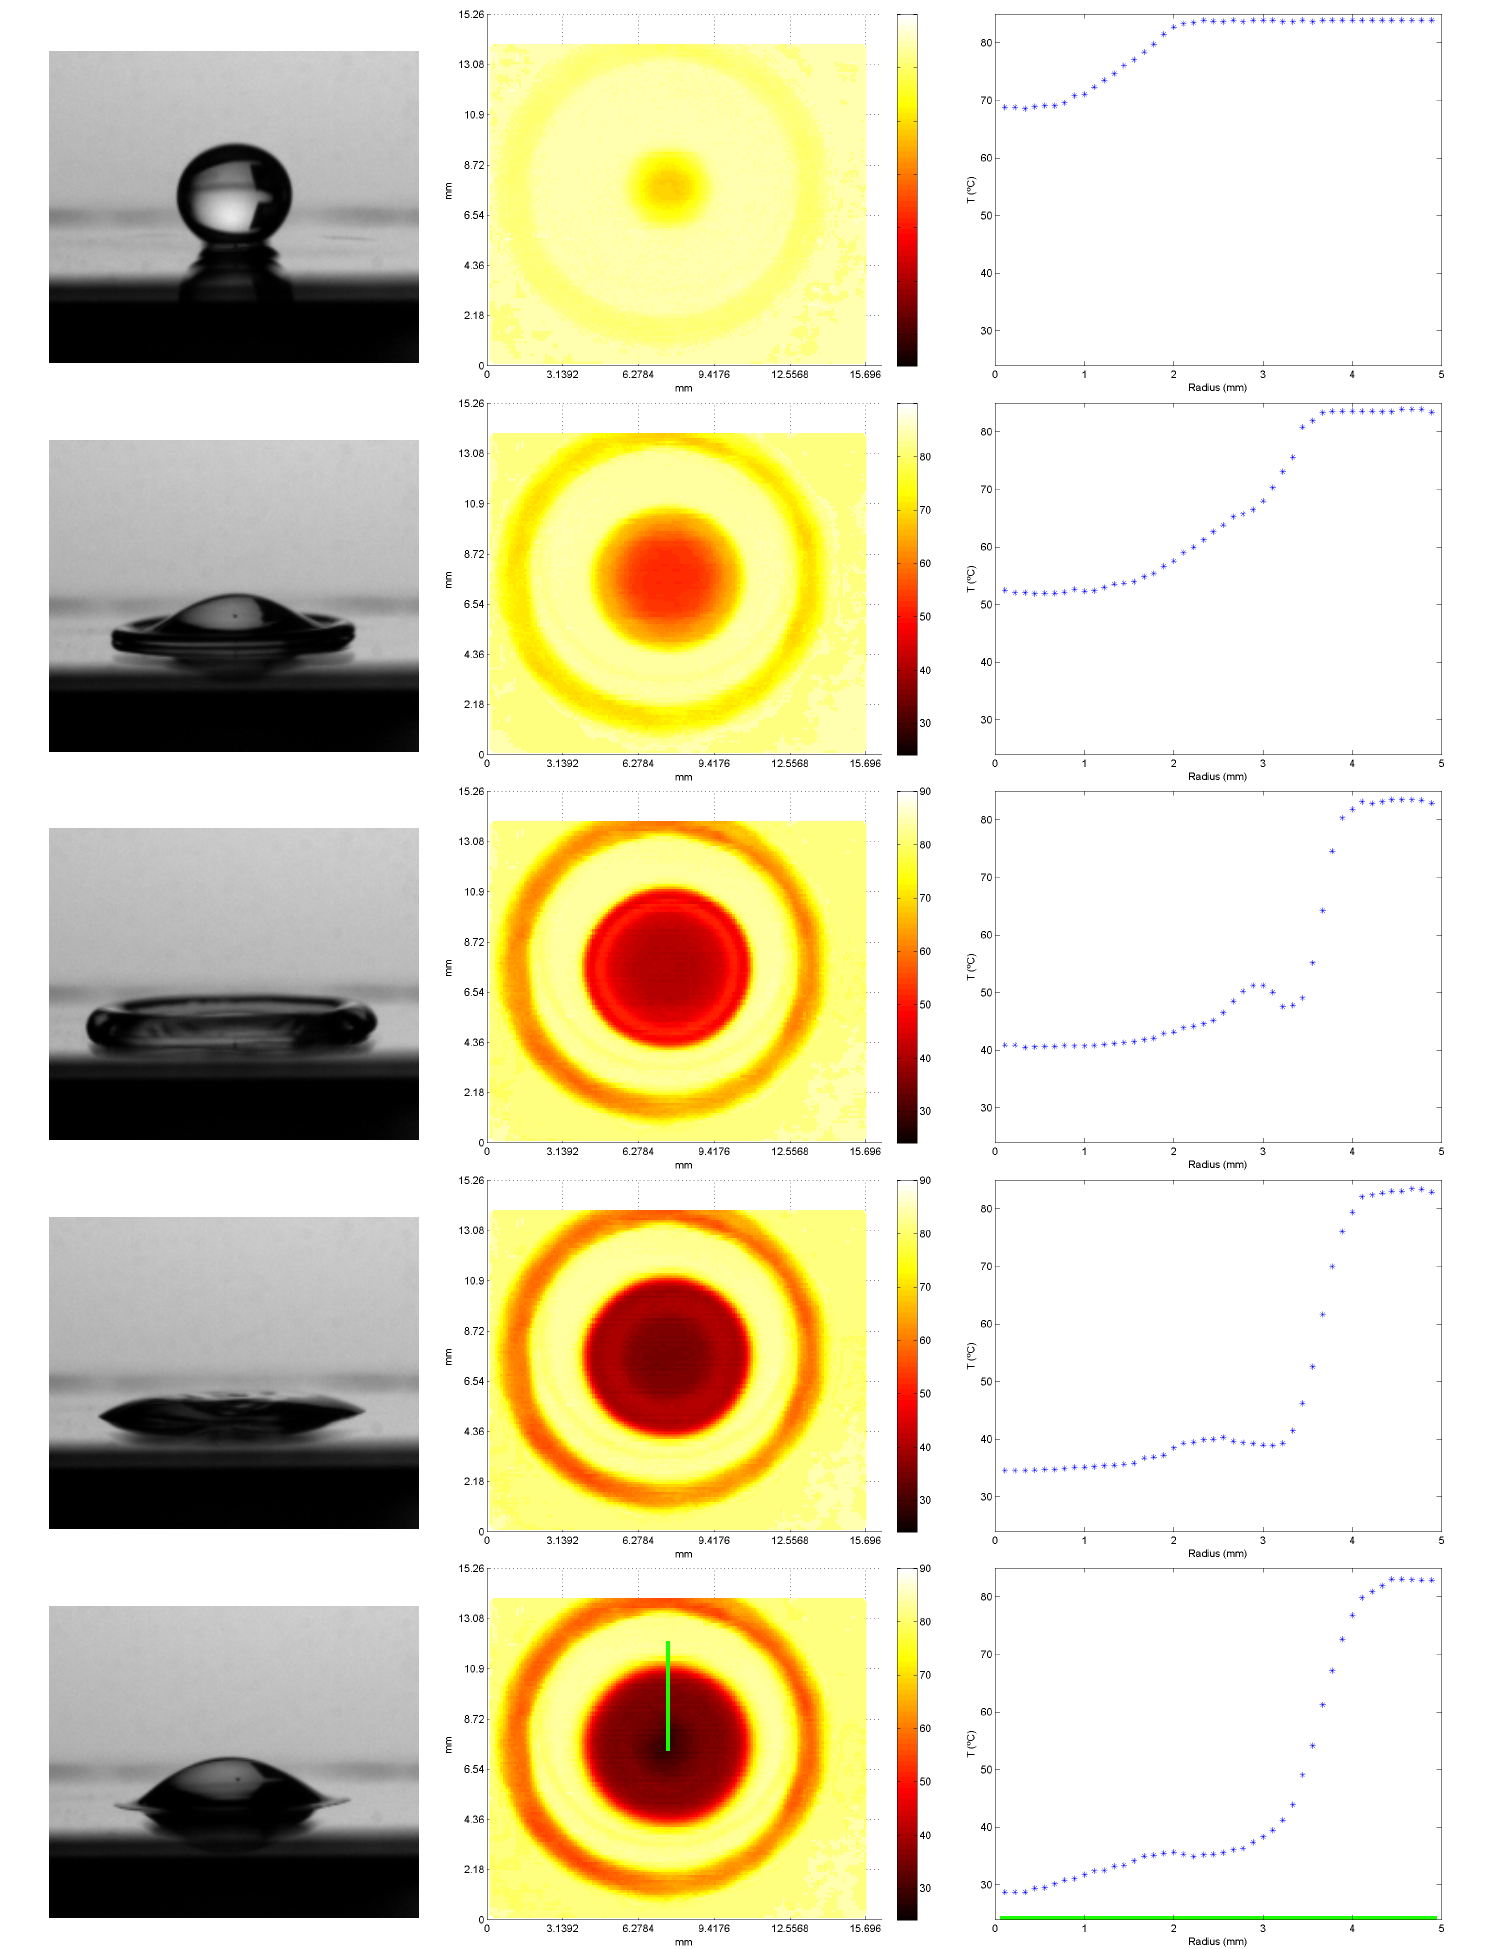
\includegraphics[width=1\linewidth]{Figures/5.Chapter/IRvsHR.png}
\caption{Comparison between High Speed camera images and Infra Red images for 0.8m/s and 80ºC at 0, 2, 6, 12 and 22 ms after the first contact on a hydrophilic surface}
\label{fig:irvshr}
\end{figure}

\par One important objective of this work is to use the high-speed camera to compare physical phenomena with thermal phenomena. The results were put together in Figure \ref{fig:irvshr}. In this figure it is possible to see some of the stages of a droplet impact. Analyzing the images, it's observable the physical phenomena that have an impact on heat transfer. During the spreading, the interior ring in the temperature maps, presented in the third and fourth images, reflect the presence of the wave formed during the spreading. When this wave reaches maximum diameter it reverses in the recoiling phase. The thickness of the water layer is smaller right before the wave. In this area there is less heat removal. So, as expected, one can see a ring of higher temperatures, and a slope in the plot. After the recoiling phase the droplet starts to stabilize, and due to it's hemispherical shape the heat flux is higher at the center, so the temperature is lower in the center.

\subsection{Velocity Influence}

\par For an hidrophilic surface, results were taken for different velocities: 0.8 m/s, 2 m/s. The obvious difference is in the spreading diameter, which is directly influenced by the impact velocity. This can be seen in Figure \label{fig:irvshr}. One of the differences is the fingering, that only happens for 2 m/s (at t= 6ms). The height of the lamela is also smaller for this velocity.

\begin{figure}[h]
\centering
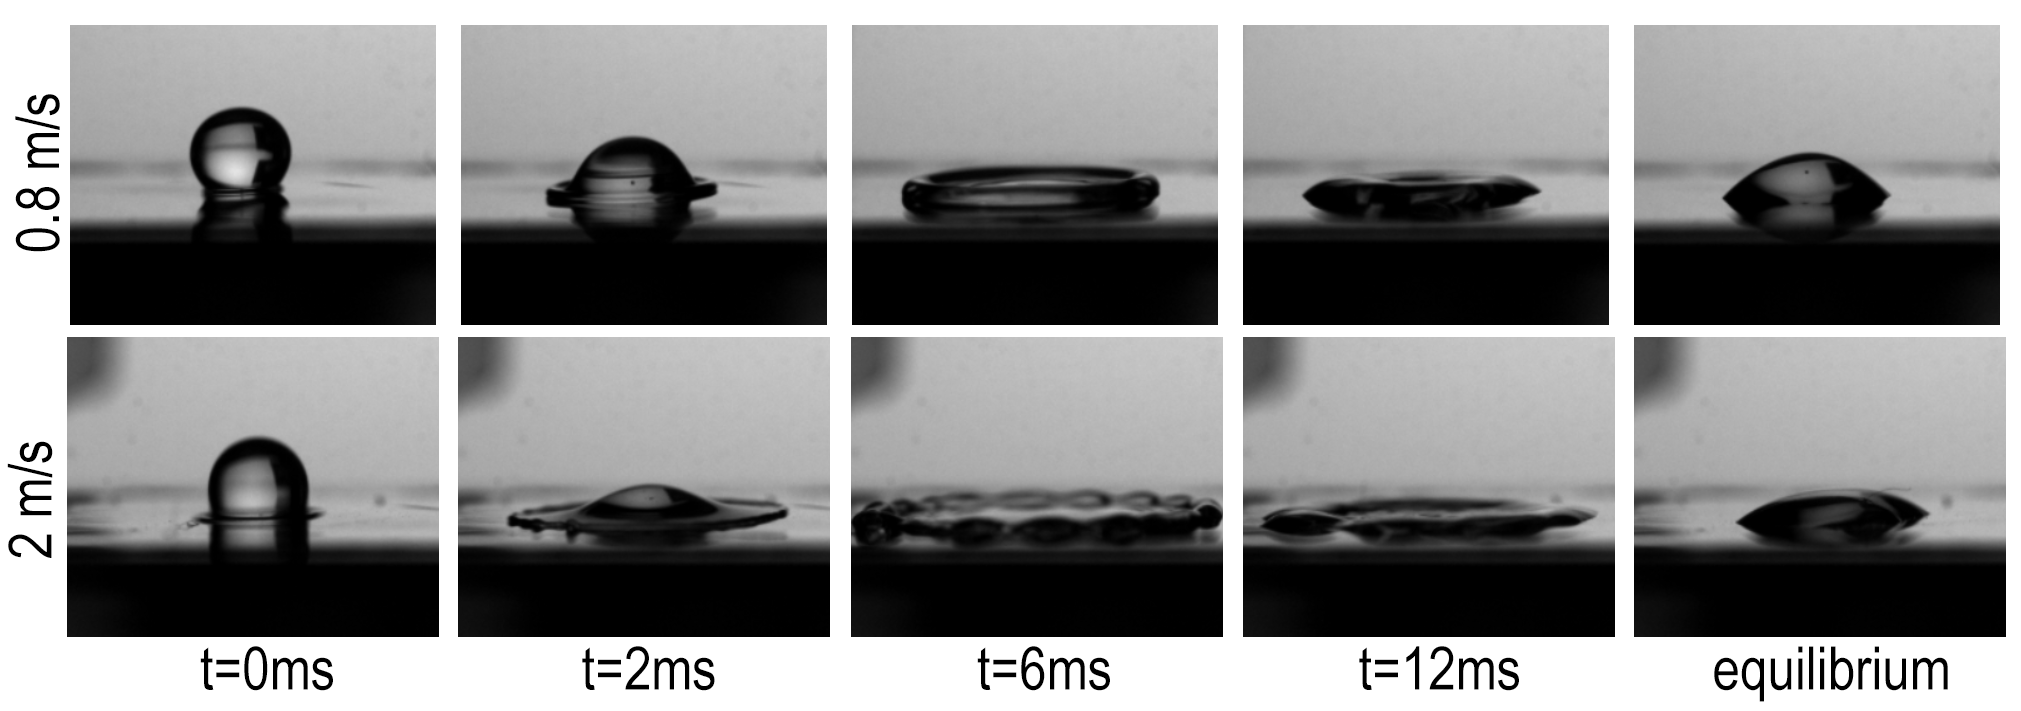
\includegraphics[width=1\linewidth]{Figures/5.Chapter/hsspeed.png}
\caption{Velocity HS images comparison for a hydrophilic surface at 100ºC}
\label{fig:irvshr}
\end{figure}


\par Using the high speed camera it was possible to extract the droplet diameter for each frame, with the help of a code developed previously by Tomás Valente. The comparison between the spreading factor of each velocity can be seen in Figure \ref{fig:diameter}. As expected the spreading factor grows more with a higher impact velocity.

\begin{figure}[h]
\centering
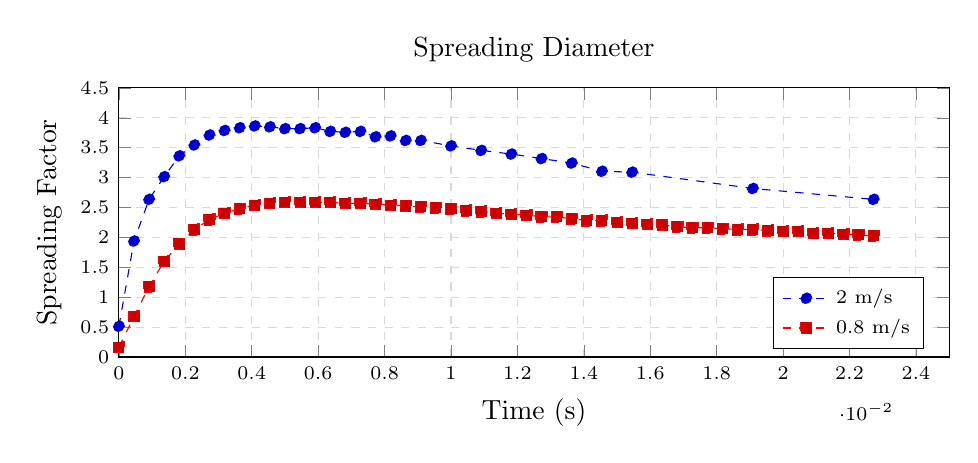
\begin{tikzpicture}
\begin{axis}[
	title = {Spreading Diameter},
    tick label style={font=\scriptsize},
    legend style={font=\scriptsize,/tikz/column 2/.style={column sep=5pt},},
    %legend columns=2,
    legend cell align=left,
	legend pos =south east,
    grid=major, % Display a grid
    grid style={dashed,gray!30}, % Set the style
    xlabel={Time (s)},
    ylabel={Spreading Factor}, 
    ymin = 0, ymax = 4.5,
    ytick={0,0.5,...,4.5},
    %yticklabels={300,325,350,375,400,425,450,475,500,525},
    xmin = 0, xmax = 0.025,
    %ytick={0,1600,...,11200},
    %yticklabel style={
    %    /pgf/number format/fixed,
    %    /pgf/number format/precision=5},
	%scaled y ticks=false,
    width=1\textwidth, height=5cm,
    cycle list name= color
    ]
\addplot+[dashed]
coordinates {(	0	,	0.515151515	)
(	0.000454545	,	1.939393939	)
(	0.000909091	,	2.636363636	)
(	0.001363636	,	3.015151515	)
(	0.001818182	,	3.363636364	)
(	0.002272727	,	3.545454545	)
(	0.002727273	,	3.712121212	)
(	0.003181818	,	3.787878788	)
(	0.003636364	,	3.833333333	)
(	0.004090909	,	3.863636364	)
(	0.004545455	,	3.848484848	)
(	0.005	,	3.818181818	)
(	0.005454545	,	3.818181818	)
(	0.005909091	,	3.833333333	)
(	0.006363636	,	3.772727273	)
(	0.006818182	,	3.757575758	)
(	0.007272727	,	3.772727273	)
(	0.007727273	,	3.681818182	)
(	0.008181818	,	3.696969697	)
(	0.008636364	,	3.621212121	)
(	0.009090909	,	3.621212121	)
(	0.01	,	3.53030303	)
(	0.010909091	,	3.454545455	)
(	0.011818182	,	3.393939394	)
(	0.012727273	,	3.318181818	)
(	0.013636364	,	3.242424242	)
(	0.014545455	,	3.106060606	)
(	0.015454545	,	3.090909091	)
(	0.019090909	,	2.818181818	)
(	0.022727273	,	2.636363636	)
};
\addlegendentry{2 m/s}

\addplot+[dashed]
coordinates {(	0	,	0.166303558	)
(	0.000454545	,	0.680332739	)
(	0.000909091	,	1.179243415	)
(	0.001363636	,	1.602561563	)
(	0.001818182	,	1.889813164	)
(	0.002272727	,	2.131709249	)
(	0.002727273	,	2.298012808	)
(	0.003181818	,	2.403842345	)
(	0.003636364	,	2.479434872	)
(	0.004090909	,	2.539908893	)
(	0.004545455	,	2.570145903	)
(	0.005	,	2.585264409	)
(	0.005454545	,	2.585264409	)
(	0.005909091	,	2.585264409	)
(	0.006363636	,	2.585264409	)
(	0.006818182	,	2.570145903	)
(	0.007272727	,	2.570145903	)
(	0.007727273	,	2.555027398	)
(	0.008181818	,	2.539908893	)
(	0.008636364	,	2.524790388	)
(	0.009090909	,	2.509671882	)
(	0.009545455	,	2.494553377	)
(	0.01	,	2.479434872	)
(	0.010454545	,	2.449197861	)
(	0.010909091	,	2.434079356	)
(	0.011363636	,	2.403842345	)
(	0.011818182	,	2.38872384	)
(	0.012272727	,	2.373605334	)
(	0.012727273	,	2.343368324	)
(	0.013181818	,	2.343368324	)
(	0.013636364	,	2.313131313	)
(	0.014090909	,	2.282894303	)
(	0.014545455	,	2.282894303	)
(	0.015	,	2.252657292	)
(	0.015454545	,	2.237538787	)
(	0.015909091	,	2.222420281	)
(	0.016363636	,	2.207301776	)
(	0.016818182	,	2.177064765	)
(	0.017272727	,	2.16194626	)
(	0.017727273	,	2.16194626	)
(	0.018181818	,	2.146827755	)
(	0.018636364	,	2.131709249	)
(	0.019090909	,	2.131709249	)
(	0.019545455	,	2.116590744	)
(	0.02	,	2.101472239	)
(	0.020454545	,	2.101472239	)
(	0.020909091	,	2.071235228	)
(	0.021363636	,	2.071235228	)
(	0.021818182	,	2.056116723	)
(	0.022272727	,	2.040998217	)
(	0.022727273	,	2.025879712	)
};
\addlegendentry{0.8 m/s}

\end{axis}
\end{tikzpicture}
\caption{Comparison between the spreading factor of each velocity}
\label{fig:diameter}
\end{figure}

\par Lets now take a look at the influence of the velocity in the temperature field. In Figure \ref{fig:speed1}, the average of all experiments made for both velocity values at 100ºC is presented for comparison. The temperature at the center of the droplet is similar during the spreading (3ms and 13 ms). The temperature at the droplet center drops more intensely in the lower velocity. This is justified by the height difference, also noticeable in the last panel of Figure \ref{fig:irvshr}. Looking at the shape of the curves, one can observe their similarity. This may be a signal of the time in which the phenomena occur is mostly independent of the impact velocity. Note that the curves have close temperatures in the center area and also that the lower velocity tests show always higher temperatures at the same point than the higher velocity ones outside the center. With this in mind, it's safe to assume that the higher velocity droplet removed more heat from the foil.

\begin{figure}[h]
\centering
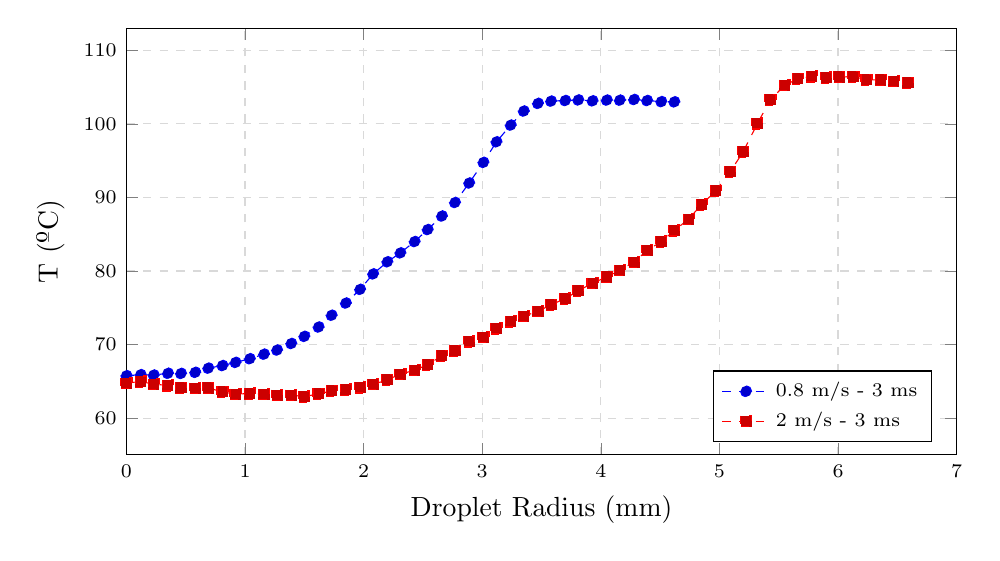
\begin{tikzpicture}
\begin{axis}[
	%title = {107 ºC || $T_{amb}=24$},
    tick label style={font=\scriptsize},
    legend style={font=\scriptsize,/tikz/column 2/.style={column sep=5pt},},
    %legend columns=2,
    legend cell align=left,
	legend pos =south east,
    grid=major, % Display a grid
    grid style={dashed,gray!30}, % Set the style
    xlabel={Droplet Radius (mm)},
    ylabel={T (ºC)}, 
    ymin = 55, ymax = 113,
    ytick={60,70,...,100,110},
    %yticklabels={300,325,350,375,400,425,450,475,500,525},
    xmin = 0, xmax = 7,
    %ytick={0,1600,...,11200},
    %yticklabel style={
    %    /pgf/number format/fixed,
    %    /pgf/number format/precision=5},
	%scaled y ticks=false,
    width=1\textwidth, height=7cm,
    cycle list name= color
    ]
\addplot+[dashed]
coordinates {(	0	,	65.76	)
(	0.12	,	65.9	)
(	0.23	,	65.85	)
(	0.35	,	66.09	)
(	0.46	,	66.07	)
(	0.58	,	66.22	)
(	0.69	,	66.79	)
(	0.81	,	67.14	)
(	0.92	,	67.57	)
(	1.04	,	68.07	)
(	1.16	,	68.69	)
(	1.27	,	69.25	)
(	1.39	,	70.14	)
(	1.5	,	71.11	)
(	1.62	,	72.38	)
(	1.73	,	73.98	)
(	1.85	,	75.64	)
(	1.97	,	77.5	)
(	2.08	,	79.6	)
(	2.2	,	81.25	)
(	2.31	,	82.46	)
(	2.43	,	84	)
(	2.54	,	85.63	)
(	2.66	,	87.47	)
(	2.77	,	89.31	)
(	2.89	,	91.96	)
(	3.01	,	94.76	)
(	3.12	,	97.56	)
(	3.24	,	99.83	)
(	3.35	,	101.74	)
(	3.47	,	102.78	)
(	3.58	,	103.09	)
(	3.7	,	103.17	)
(	3.81	,	103.25	)
(	3.93	,	103.13	)
(	4.05	,	103.23	)
(	4.16	,	103.22	)
(	4.28	,	103.31	)
(	4.39	,	103.17	)
(	4.51	,	103.02	)
(	4.62	,	102.99	)
};
\addlegendentry{0.8 m/s - 3 ms}

\addplot+[dashed]
coordinates {(	0	,	64.76	)
(	0.12	,	64.97	)
(	0.23	,	64.61	)
(	0.35	,	64.44	)
(	0.46	,	64.13	)
(	0.58	,	64.08	)
(	0.69	,	64.09	)
(	0.81	,	63.56	)
(	0.92	,	63.26	)
(	1.04	,	63.34	)
(	1.16	,	63.22	)
(	1.27	,	63.12	)
(	1.39	,	63.12	)
(	1.5	,	62.93	)
(	1.62	,	63.29	)
(	1.73	,	63.7	)
(	1.85	,	63.88	)
(	1.97	,	64.17	)
(	2.08	,	64.58	)
(	2.2	,	65.21	)
(	2.31	,	65.97	)
(	2.43	,	66.51	)
(	2.54	,	67.27	)
(	2.66	,	68.47	)
(	2.77	,	69.17	)
(	2.89	,	70.41	)
(	3.01	,	71.01	)
(	3.12	,	72.19	)
(	3.24	,	73.14	)
(	3.35	,	73.85	)
(	3.47	,	74.52	)
(	3.58	,	75.4	)
(	3.7	,	76.25	)
(	3.81	,	77.3	)
(	3.93	,	78.35	)
(	4.05	,	79.18	)
(	4.16	,	80.08	)
(	4.28	,	81.21	)
(	4.39	,	82.8	)
(	4.51	,	84	)
(	4.62	,	85.5	)
(	4.74	,	87.06	)
(	4.85	,	89.03	)
(	4.97	,	90.91	)
(	5.09	,	93.49	)
(	5.2	,	96.19	)
(	5.32	,	100.05	)
(	5.43	,	103.28	)
(	5.55	,	105.25	)
(	5.66	,	106.11	)
(	5.78	,	106.44	)
(	5.9	,	106.29	)
(	6.01	,	106.37	)
(	6.13	,	106.42	)
(	6.24	,	106	)
(	6.36	,	105.96	)
(	6.47	,	105.78	)
(	6.59	,	105.59	)
};
\addlegendentry{2 m/s - 3 ms}

\end{axis}
\end{tikzpicture}
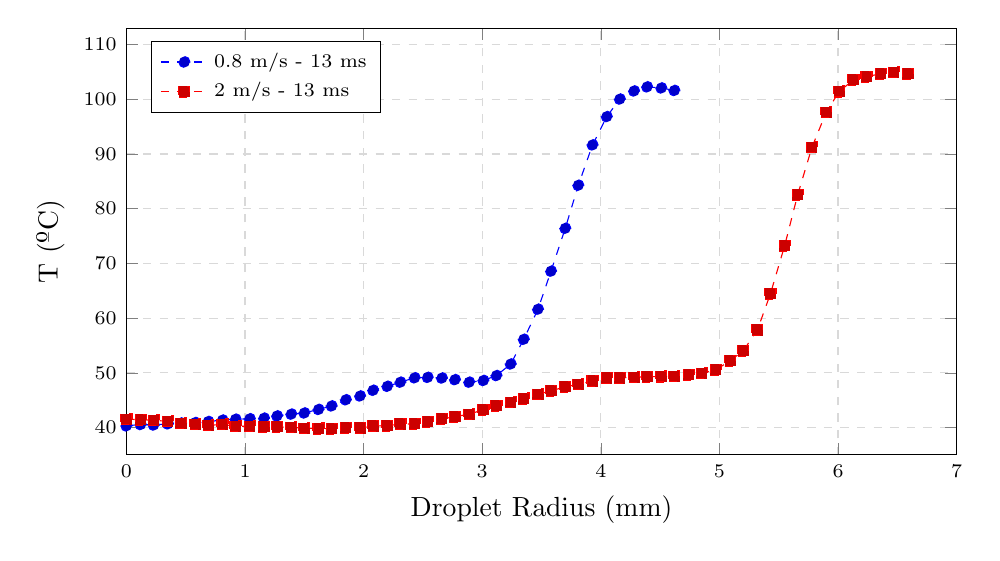
\begin{tikzpicture}
\begin{axis}[
	%title = {107 ºC || $T_{amb}=24$},
    tick label style={font=\scriptsize},
    legend style={font=\scriptsize,/tikz/column 2/.style={column sep=5pt},},
    %legend columns=2,
    legend cell align=left,
	legend pos =north west,
    grid=major, % Display a grid
    grid style={dashed,gray!30}, % Set the style
    xlabel={Droplet Radius (mm)},
    ylabel={T (ºC)}, 
    ymin = 35, ymax = 113,
    ytick={30,40,...,100,110},
    %yticklabels={300,325,350,375,400,425,450,475,500,525},
    xmin = 0, xmax = 7,
    %ytick={0,1600,...,11200},
    %yticklabel style={
    %    /pgf/number format/fixed,
    %    /pgf/number format/precision=5},
	%scaled y ticks=false,
    width=1\textwidth, height=7cm,
    cycle list name= color
    ]
\addplot+[dashed]
coordinates {(	0	,	40.31	)
(	0.12	,	40.55	)
(	0.23	,	40.46	)
(	0.35	,	40.67	)
(	0.46	,	40.82	)
(	0.58	,	40.91	)
(	0.69	,	41.1	)
(	0.81	,	41.36	)
(	0.92	,	41.52	)
(	1.04	,	41.6	)
(	1.16	,	41.71	)
(	1.27	,	42.12	)
(	1.39	,	42.45	)
(	1.5	,	42.66	)
(	1.62	,	43.31	)
(	1.73	,	43.95	)
(	1.85	,	45.07	)
(	1.97	,	45.77	)
(	2.08	,	46.81	)
(	2.2	,	47.54	)
(	2.31	,	48.29	)
(	2.43	,	49.09	)
(	2.54	,	49.17	)
(	2.66	,	49.05	)
(	2.77	,	48.75	)
(	2.89	,	48.29	)
(	3.01	,	48.6	)
(	3.12	,	49.5	)
(	3.24	,	51.61	)
(	3.35	,	56.13	)
(	3.47	,	61.63	)
(	3.58	,	68.59	)
(	3.7	,	76.42	)
(	3.81	,	84.29	)
(	3.93	,	91.67	)
(	4.05	,	96.84	)
(	4.16	,	100.05	)
(	4.28	,	101.53	)
(	4.39	,	102.28	)
(	4.51	,	102.08	)
(	4.62	,	101.62	)
};
\addlegendentry{0.8 m/s - 13 ms}

\addplot+[dashed]
coordinates {(	0	,	41.51	)
(	0.12	,	41.44	)
(	0.23	,	41.31	)
(	0.35	,	41.14	)
(	0.46	,	40.77	)
(	0.58	,	40.61	)
(	0.69	,	40.39	)
(	0.81	,	40.57	)
(	0.92	,	40.22	)
(	1.04	,	40.24	)
(	1.16	,	40.11	)
(	1.27	,	40.11	)
(	1.39	,	40.05	)
(	1.5	,	39.87	)
(	1.62	,	39.81	)
(	1.73	,	39.79	)
(	1.85	,	39.95	)
(	1.97	,	39.91	)
(	2.08	,	40.28	)
(	2.2	,	40.34	)
(	2.31	,	40.64	)
(	2.43	,	40.65	)
(	2.54	,	41.02	)
(	2.66	,	41.57	)
(	2.77	,	41.97	)
(	2.89	,	42.46	)
(	3.01	,	43.23	)
(	3.12	,	43.95	)
(	3.24	,	44.59	)
(	3.35	,	45.3	)
(	3.47	,	46.08	)
(	3.58	,	46.71	)
(	3.7	,	47.43	)
(	3.81	,	47.91	)
(	3.93	,	48.5	)
(	4.05	,	49.05	)
(	4.16	,	49.05	)
(	4.28	,	49.21	)
(	4.39	,	49.27	)
(	4.51	,	49.33	)
(	4.62	,	49.37	)
(	4.74	,	49.62	)
(	4.85	,	49.94	)
(	4.97	,	50.54	)
(	5.09	,	52.22	)
(	5.2	,	54.01	)
(	5.32	,	57.83	)
(	5.43	,	64.46	)
(	5.55	,	73.26	)
(	5.66	,	82.58	)
(	5.78	,	91.23	)
(	5.9	,	97.63	)
(	6.01	,	101.44	)
(	6.13	,	103.55	)
(	6.24	,	104.15	)
(	6.36	,	104.67	)
(	6.47	,	104.97	)
(	6.59	,	104.65	)
};
\addlegendentry{2 m/s - 13 ms}
\end{axis}
\end{tikzpicture}
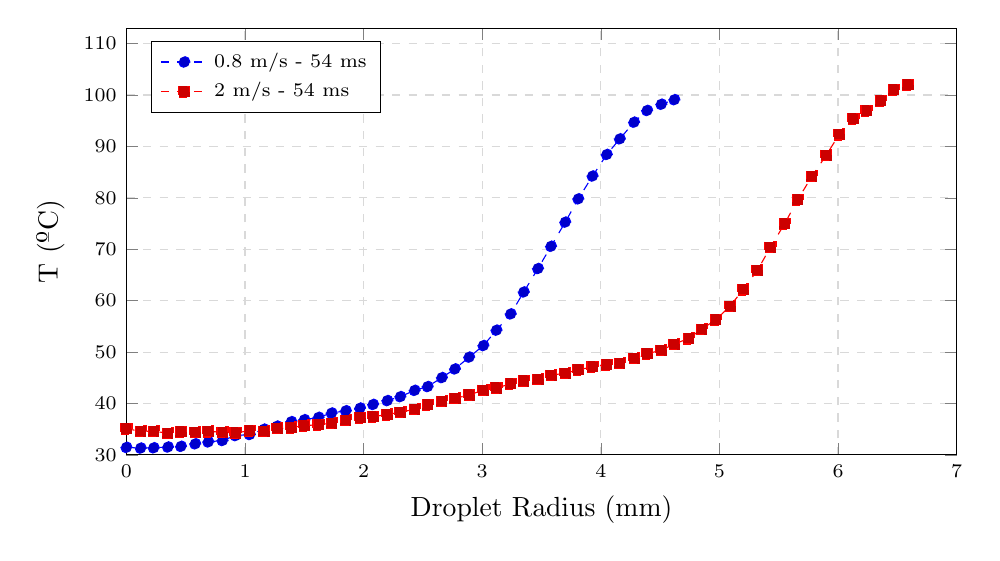
\begin{tikzpicture}
\begin{axis}[
	%
    tick label style={font=\scriptsize},
    legend style={font=\scriptsize,/tikz/column 2/.style={column sep=5pt},},
    %legend columns=2,
    legend cell align=left,
	legend pos =north west,
    grid=major, % Display a grid
    grid style={dashed,gray!30}, % Set the style
    xlabel={Droplet Radius (mm)},
    ylabel={T (ºC)}, 
    ymin = 30, ymax = 113,
    ytick={30,40,...,100,110},
    %yticklabels={300,325,350,375,400,425,450,475,500,525},
    xmin = 0, xmax = 7,
    %ytick={0,1600,...,11200},
    %yticklabel style={
    %    /pgf/number format/fixed,
    %    /pgf/number format/precision=5},
	%scaled y ticks=false,
    width=1\textwidth, height=7cm,
    cycle list name= color
    ]
\addplot+[dashed]
coordinates {(	0	,	31.46	)
(	0.12	,	31.32	)
(	0.23	,	31.38	)
(	0.35	,	31.53	)
(	0.46	,	31.66	)
(	0.58	,	32.15	)
(	0.69	,	32.52	)
(	0.81	,	32.8	)
(	0.92	,	33.75	)
(	1.04	,	33.96	)
(	1.16	,	35	)
(	1.27	,	35.59	)
(	1.39	,	36.46	)
(	1.5	,	36.84	)
(	1.62	,	37.3	)
(	1.73	,	38.14	)
(	1.85	,	38.58	)
(	1.97	,	39.1	)
(	2.08	,	39.81	)
(	2.2	,	40.56	)
(	2.31	,	41.33	)
(	2.43	,	42.55	)
(	2.54	,	43.29	)
(	2.66	,	45.03	)
(	2.77	,	46.72	)
(	2.89	,	49.02	)
(	3.01	,	51.27	)
(	3.12	,	54.26	)
(	3.24	,	57.42	)
(	3.35	,	61.69	)
(	3.47	,	66.25	)
(	3.58	,	70.58	)
(	3.7	,	75.28	)
(	3.81	,	79.81	)
(	3.93	,	84.25	)
(	4.05	,	88.44	)
(	4.16	,	91.48	)
(	4.28	,	94.72	)
(	4.39	,	97	)
(	4.51	,	98.21	)
(	4.62	,	99.1	)
};
\addlegendentry{0.8 m/s - 54 ms}

\addplot+[dashed]
coordinates {(	0	,	35.05	)
(	0.12	,	34.63	)
(	0.23	,	34.58	)
(	0.35	,	34.24	)
(	0.46	,	34.48	)
(	0.58	,	34.4	)
(	0.69	,	34.56	)
(	0.81	,	34.42	)
(	0.92	,	34.26	)
(	1.04	,	34.72	)
(	1.16	,	34.6	)
(	1.27	,	35.17	)
(	1.39	,	35.31	)
(	1.5	,	35.71	)
(	1.62	,	35.84	)
(	1.73	,	36.19	)
(	1.85	,	36.73	)
(	1.97	,	37.22	)
(	2.08	,	37.44	)
(	2.2	,	37.85	)
(	2.31	,	38.32	)
(	2.43	,	38.85	)
(	2.54	,	39.73	)
(	2.66	,	40.45	)
(	2.77	,	41.01	)
(	2.89	,	41.65	)
(	3.01	,	42.6	)
(	3.12	,	43.01	)
(	3.24	,	43.82	)
(	3.35	,	44.37	)
(	3.47	,	44.7	)
(	3.58	,	45.48	)
(	3.7	,	45.91	)
(	3.81	,	46.53	)
(	3.93	,	47.14	)
(	4.05	,	47.55	)
(	4.16	,	47.86	)
(	4.28	,	48.81	)
(	4.39	,	49.67	)
(	4.51	,	50.37	)
(	4.62	,	51.56	)
(	4.74	,	52.65	)
(	4.85	,	54.44	)
(	4.97	,	56.31	)
(	5.09	,	58.93	)
(	5.2	,	62.17	)
(	5.32	,	65.89	)
(	5.43	,	70.41	)
(	5.55	,	74.98	)
(	5.66	,	79.66	)
(	5.78	,	84.19	)
(	5.9	,	88.29	)
(	6.01	,	92.34	)
(	6.13	,	95.38	)
(	6.24	,	96.93	)
(	6.36	,	98.86	)
(	6.47	,	101.02	)
(	6.59	,	102.02	)
};
\addlegendentry{2 m/s - 54 ms}

\end{axis}
\end{tikzpicture}
\caption{Average temperature along the radius between the 5 experiments of both velocity values at 100ºC}
\label{fig:speed1}
\end{figure}

\subsection{Temperature Influence}

\par This section will address the relative temperature drop in the foil for the tested temperatures. The temperatures had to be adimensionalized  so that they could be compared. \\

\par This analysis, for a fixed impact velocity of 0.8 m/s, can be seen in Figure \ref{fig:temp}. In this figure one can see that for the different initial temperatures, the relative temperature drop is very similar in the center, but has a significant difference in the edge area. This may be the cause of different diameters at that time, which can shift the curve.

\par This is a confirmation for the effectiveness of the  weighted background test. Because the curves vary so little for the different temperatures, one can assume that the relative temperature drop is constant and so, even if the background has different temperatures at its initial stage it is possible to assume a constant temperature if this technique is used.

\begin{figure}[h]
\centering
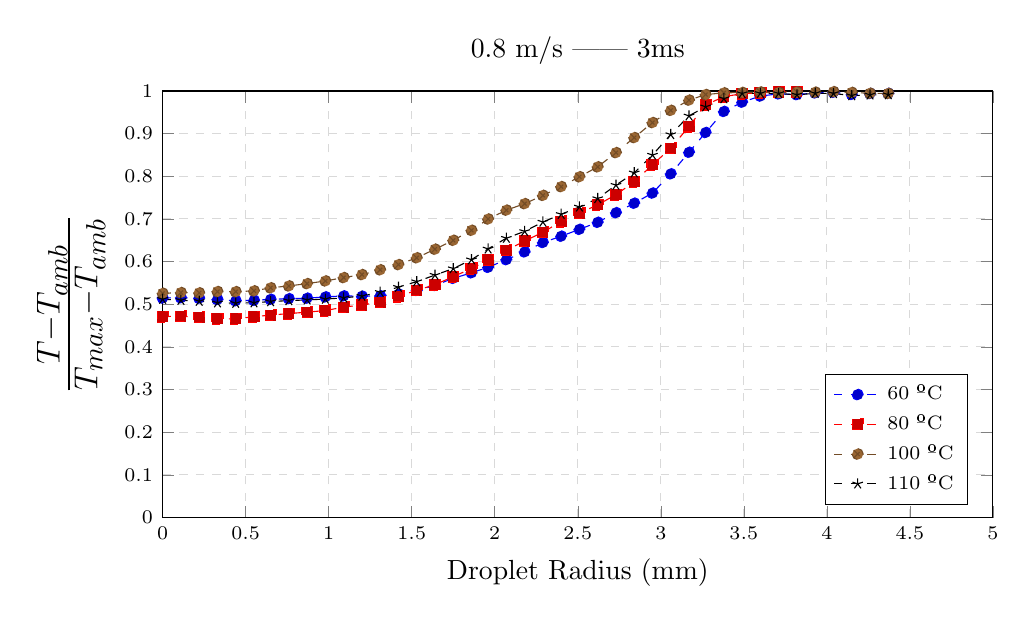
\begin{tikzpicture}
\begin{axis}[
	title = {0.8 m/s || 3ms},
    tick label style={font=\scriptsize},
    legend style={font=\scriptsize,/tikz/column 2/.style={column sep=5pt},},
    %legend columns=2,
    legend cell align=left,
	legend pos =south east,
    grid=major, % Display a grid
    grid style={dashed,gray!30}, % Set the style
    xlabel={Droplet Radius (mm)},
    ylabel={\LARGE{$\frac{T-T_{amb}}{T_{max}-T_{amb}}$}}, 
    ymin = 0, ymax = 1,
    ytick={0,0.1,...,1},
    %yticklabels={300,325,350,375,400,425,450,475,500,525},
    xmin = 0, xmax = 5,
    %ytick={0,1600,...,11200},
    %yticklabel style={
    %    /pgf/number format/fixed,
    %    /pgf/number format/precision=5},
	%scaled y ticks=false,
    width=1\textwidth, 
    height=7cm,
    cycle list name= color
    ]
\addplot+[dashed]
coordinates {(	0	,	0.514798887	)
(	0.11	,	0.515304832	)
(	0.22	,	0.514292942	)
(	0.33	,	0.511257273	)
(	0.44	,	0.508221604	)
(	0.55	,	0.509233494	)
(	0.65	,	0.511510245	)
(	0.76	,	0.51302808	)
(	0.87	,	0.514292942	)
(	0.98	,	0.517328611	)
(	1.09	,	0.519605363	)
(	1.2	,	0.518846446	)
(	1.31	,	0.519858335	)
(	1.42	,	0.523652922	)
(	1.53	,	0.532506957	)
(	1.64	,	0.544143688	)
(	1.75	,	0.560839868	)
(	1.86	,	0.573741462	)
(	1.96	,	0.586643056	)
(	2.07	,	0.604604098	)
(	2.18	,	0.622818113	)
(	2.29	,	0.644826714	)
(	2.4	,	0.659499115	)
(	2.51	,	0.67568935	)
(	2.62	,	0.692132558	)
(	2.73	,	0.714647103	)
(	2.84	,	0.736908677	)
(	2.95	,	0.760688085	)
(	3.06	,	0.805717177	)
(	3.17	,	0.856311662	)
(	3.27	,	0.902605616	)
(	3.38	,	0.951935239	)
(	3.49	,	0.973690868	)
(	3.6	,	0.988110296	)
(	3.71	,	0.993169744	)
(	3.82	,	0.991398938	)
(	3.93	,	0.995446496	)
(	4.04	,	0.996964331	)
(	4.15	,	0.991904882	)
(	4.26	,	0.993928662	)
(	4.37	,	0.994181634	)
};
\addlegendentry{60 ºC}

\addplot+[dashed]
coordinates {(	0	,	0.471055243	)
(	0.11	,	0.472213033	)
(	0.22	,	0.469401257	)
(	0.33	,	0.465597089	)
(	0.44	,	0.466093285	)
(	0.55	,	0.470724446	)
(	0.65	,	0.474694013	)
(	0.76	,	0.478167383	)
(	0.87	,	0.481640754	)
(	0.98	,	0.485279524	)
(	1.09	,	0.493384056	)
(	1.2	,	0.498346014	)
(	1.31	,	0.504961958	)
(	1.42	,	0.518193847	)
(	1.53	,	0.532914324	)
(	1.64	,	0.545815415	)
(	1.75	,	0.564836255	)
(	1.86	,	0.583691697	)
(	1.96	,	0.603704929	)
(	2.07	,	0.626364539	)
(	2.18	,	0.648362554	)
(	2.29	,	0.668706583	)
(	2.4	,	0.69401257	)
(	2.51	,	0.713695005	)
(	2.62	,	0.733046642	)
(	2.73	,	0.756864042	)
(	2.84	,	0.786966589	)
(	2.95	,	0.826993053	)
(	3.06	,	0.865861727	)
(	3.17	,	0.916804499	)
(	3.27	,	0.967251075	)
(	3.38	,	0.986602713	)
(	3.49	,	0.993549454	)
(	3.6	,	0.995699636	)
(	3.71	,	0.997519021	)
(	3.82	,	0.998346014	)
};
\addlegendentry{80 ºC}

\addplot+[dashed]
coordinates {(	0	,	0.525613593	)
(	0.11	,	0.527375708	)
(	0.22	,	0.526746381	)
(	0.33	,	0.529767149	)
(	0.44	,	0.529515419	)
(	0.55	,	0.531403398	)
(	0.65	,	0.538577722	)
(	0.76	,	0.542983008	)
(	0.87	,	0.548395217	)
(	0.98	,	0.554688483	)
(	1.09	,	0.562492133	)
(	1.2	,	0.569540592	)
(	1.31	,	0.580742605	)
(	1.42	,	0.592951542	)
(	1.53	,	0.608936438	)
(	1.64	,	0.62907489	)
(	1.75	,	0.649968534	)
(	1.86	,	0.673379484	)
(	1.96	,	0.699811202	)
(	2.07	,	0.72057898	)
(	2.18	,	0.735808685	)
(	2.29	,	0.755191945	)
(	2.4	,	0.775707992	)
(	2.51	,	0.798867212	)
(	2.62	,	0.822026432	)
(	2.73	,	0.855380743	)
(	2.84	,	0.890623033	)
(	2.95	,	0.925865324	)
(	3.06	,	0.954436753	)
(	3.17	,	0.97847703	)
(	3.27	,	0.991567023	)
(	3.38	,	0.995468848	)
(	3.49	,	0.996475771	)
(	3.6	,	0.997482694	)
(	3.71	,	0.99597231	)
(	3.82	,	0.997230963	)
(	3.93	,	0.997105098	)
(	4.04	,	0.998237885	)
(	4.15	,	0.996475771	)
(	4.26	,	0.994587791	)
(	4.37	,	0.994210195	)
};
\addlegendentry{100 ºC}

\addplot+[dashed]
coordinates {(	0	,	0.511852408	)
(	0.11	,	0.509385391	)
(	0.22	,	0.507240159	)
(	0.33	,	0.503486002	)
(	0.44	,	0.502520648	)
(	0.55	,	0.503593264	)
(	0.65	,	0.506274804	)
(	0.76	,	0.50863456	)
(	0.87	,	0.510243484	)
(	0.98	,	0.512174193	)
(	1.09	,	0.515070256	)
(	1.2	,	0.519146198	)
(	1.31	,	0.528156173	)
(	1.42	,	0.540062212	)
(	1.53	,	0.553148128	)
(	1.64	,	0.568379277	)
(	1.75	,	0.583717687	)
(	1.86	,	0.60452644	)
(	1.96	,	0.62984018	)
(	2.07	,	0.654939397	)
(	2.18	,	0.670921377	)
(	2.29	,	0.692802746	)
(	2.4	,	0.710929958	)
(	2.51	,	0.728199078	)
(	2.62	,	0.747935214	)
(	2.73	,	0.779255604	)
(	2.84	,	0.808216239	)
(	2.95	,	0.849833745	)
(	3.06	,	0.897886946	)
(	3.17	,	0.941649684	)
(	3.27	,	0.962994744	)
(	3.38	,	0.981980049	)
(	3.49	,	0.99399335	)
(	3.6	,	0.994529658	)
(	3.71	,	0.994100611	)
(	3.82	,	0.990882763	)
(	3.93	,	0.994529658	)
(	4.04	,	0.994100611	)
(	4.15	,	0.989059316	)
(	4.26	,	0.990775501	)
(	4.37	,	0.99131181	)
};
\addlegendentry{110 ºC}

\end{axis}
\end{tikzpicture}
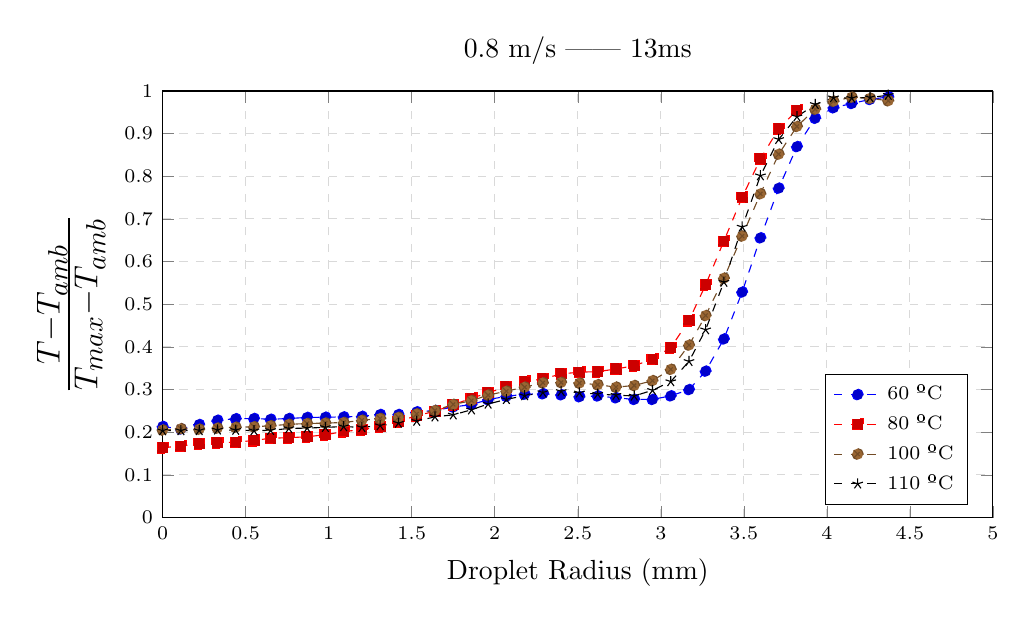
\begin{tikzpicture}
\begin{axis}[
	title = {0.8 m/s || 13ms},
    tick label style={font=\scriptsize},
    legend style={font=\scriptsize,/tikz/column 2/.style={column sep=5pt},},
    %legend columns=2,
    legend cell align=left,
	legend pos =south east,
    grid=major, % Display a grid
    grid style={dashed,gray!30}, % Set the style
    xlabel={Droplet Radius (mm)},
    ylabel={\LARGE{$\frac{T-T_{amb}}{T_{max}-T_{amb}}$}}, 
    ymin = 0, ymax = 1,
    ytick={0,0.1,...,1},
    %yticklabels={300,325,350,375,400,425,450,475,500,525},
    xmin = 0, xmax = 5,
    %ytick={0,1600,...,11200},
    %yticklabel style={
    %    /pgf/number format/fixed,
    %    /pgf/number format/precision=5},
	%scaled y ticks=false,
    width=1\textwidth, 
    height=7cm,
    cycle list name= color
    ]
\addplot+[dashed]
coordinates {(	0	,	0.213508728	)
(	0.11	,	0.207690362	)
(	0.22	,	0.218062231	)
(	0.33	,	0.228181128	)
(	0.44	,	0.231722742	)
(	0.55	,	0.232228687	)
(	0.65	,	0.23045788	)
(	0.76	,	0.232228687	)
(	0.87	,	0.234758411	)
(	0.98	,	0.235264356	)
(	1.09	,	0.236023273	)
(	1.2	,	0.237288136	)
(	1.31	,	0.241588667	)
(	1.42	,	0.241588667	)
(	1.53	,	0.247912977	)
(	1.64	,	0.250948647	)
(	1.75	,	0.259296737	)
(	1.86	,	0.26486213	)
(	1.96	,	0.276498862	)
(	2.07	,	0.284341007	)
(	2.18	,	0.289147483	)
(	2.29	,	0.290159373	)
(	2.4	,	0.287882621	)
(	2.51	,	0.283329117	)
(	2.62	,	0.285099924	)
(	2.73	,	0.280799393	)
(	2.84	,	0.277004806	)
(	2.95	,	0.277004806	)
(	3.06	,	0.285352897	)
(	3.17	,	0.300025297	)
(	3.27	,	0.343283582	)
(	3.38	,	0.418669365	)
(	3.49	,	0.52871237	)
(	3.6	,	0.655704528	)
(	3.71	,	0.772071844	)
(	3.82	,	0.869466228	)
(	3.93	,	0.935997976	)
(	4.04	,	0.960536302	)
(	4.15	,	0.970655199	)
(	4.26	,	0.980015178	)
(	4.37	,	0.986086517	)
};
\addlegendentry{60 ºC}

\addplot+[dashed]
coordinates {(	0	,	0.163910023	)
(	0.11	,	0.167714191	)
(	0.22	,	0.173337744	)
(	0.33	,	0.175487926	)
(	0.44	,	0.176645716	)
(	0.55	,	0.180780681	)
(	0.65	,	0.186073437	)
(	0.76	,	0.187231227	)
(	0.87	,	0.189546808	)
(	0.98	,	0.194177969	)
(	1.09	,	0.201786305	)
(	1.2	,	0.206086669	)
(	1.31	,	0.212537215	)
(	1.42	,	0.225107509	)
(	1.53	,	0.239000992	)
(	1.64	,	0.249090308	)
(	1.75	,	0.264803176	)
(	1.86	,	0.279689051	)
(	1.96	,	0.292590142	)
(	2.07	,	0.306152828	)
(	2.18	,	0.318888521	)
(	2.29	,	0.32500827	)
(	2.4	,	0.336751571	)
(	2.51	,	0.340886537	)
(	2.62	,	0.342044327	)
(	2.73	,	0.348329474	)
(	2.84	,	0.35593781	)
(	2.95	,	0.37148528	)
(	3.06	,	0.398445253	)
(	3.17	,	0.462123718	)
(	3.27	,	0.545650017	)
(	3.38	,	0.648197155	)
(	3.49	,	0.750909692	)
(	3.6	,	0.840555739	)
(	3.71	,	0.911346345	)
(	3.82	,	0.954515382	)
};
\addlegendentry{80 ºC}

\addplot+[dashed]
coordinates {(	0	,	0.205286344	)
(	0.11	,	0.208307111	)
(	0.22	,	0.207174323	)
(	0.33	,	0.209817495	)
(	0.44	,	0.211705475	)
(	0.55	,	0.212838263	)
(	0.65	,	0.215229704	)
(	0.76	,	0.218502203	)
(	0.87	,	0.220516048	)
(	0.98	,	0.22152297	)
(	1.09	,	0.222907489	)
(	1.2	,	0.228067967	)
(	1.31	,	0.232221523	)
(	1.42	,	0.234864695	)
(	1.53	,	0.243045941	)
(	1.64	,	0.251101322	)
(	1.75	,	0.265198238	)
(	1.86	,	0.274008811	)
(	1.96	,	0.287098804	)
(	2.07	,	0.296286973	)
(	2.18	,	0.305726872	)
(	2.29	,	0.315796098	)
(	2.4	,	0.316803021	)
(	2.51	,	0.315292637	)
(	2.62	,	0.311516677	)
(	2.73	,	0.305726872	)
(	2.84	,	0.309628697	)
(	2.95	,	0.320956576	)
(	3.06	,	0.34751416	)
(	3.17	,	0.404405286	)
(	3.27	,	0.473631215	)
(	3.38	,	0.56123348	)
(	3.49	,	0.659786029	)
(	3.6	,	0.758842039	)
(	3.71	,	0.851730648	)
(	3.82	,	0.916803021	)
(	3.93	,	0.95720579	)
(	4.04	,	0.975833858	)
(	4.15	,	0.985273757	)
(	4.26	,	0.982756451	)
(	4.37	,	0.976966646	)
};
\addlegendentry{100 ºC}

\addplot+[dashed]
coordinates {(	0	,	0.203797061	)
(	0.11	,	0.203904323	)
(	0.22	,	0.204226107	)
(	0.33	,	0.205513247	)
(	0.44	,	0.204976939	)
(	0.55	,	0.203904323	)
(	0.65	,	0.204440631	)
(	0.76	,	0.208945618	)
(	0.87	,	0.209803711	)
(	0.98	,	0.211519897	)
(	1.09	,	0.213343344	)
(	1.2	,	0.211412635	)
(	1.31	,	0.2157031	)
(	1.42	,	0.221495227	)
(	1.53	,	0.226107476	)
(	1.64	,	0.236190068	)
(	1.75	,	0.240909578	)
(	1.86	,	0.252708356	)
(	1.96	,	0.26633058	)
(	2.07	,	0.277056741	)
(	2.18	,	0.285852193	)
(	2.29	,	0.293253245	)
(	2.4	,	0.295934785	)
(	2.51	,	0.292502413	)
(	2.62	,	0.289499088	)
(	2.73	,	0.28692481	)
(	2.84	,	0.285101362	)
(	2.95	,	0.298401802	)
(	3.06	,	0.31888877	)
(	3.17	,	0.36619114	)
(	3.27	,	0.440416175	)
(	3.38	,	0.551968251	)
(	3.49	,	0.68111123	)
(	3.6	,	0.801458758	)
(	3.71	,	0.886517215	)
(	3.82	,	0.939611713	)
(	3.93	,	0.968572348	)
(	4.04	,	0.984232543	)
(	4.15	,	0.983159927	)
(	4.26	,	0.984554328	)
(	4.37	,	0.99002467	)
};
\addlegendentry{110 ºC}

\end{axis}
\end{tikzpicture}
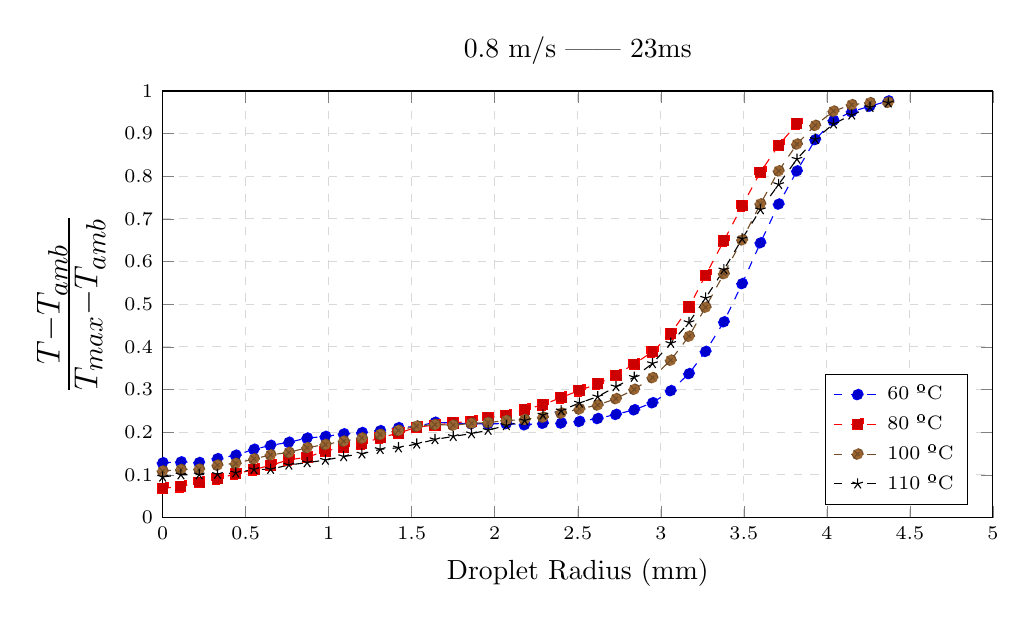
\begin{tikzpicture}
\begin{axis}[
	title = {0.8 m/s || 23ms},
    tick label style={font=\scriptsize},
    legend style={font=\scriptsize,/tikz/column 2/.style={column sep=5pt},},
    %legend columns=2,
    legend cell align=left,
	legend pos =south east,
    grid=major, % Display a grid
    grid style={dashed,gray!30}, % Set the style
    xlabel={Droplet Radius (mm)},
    ylabel={\LARGE{$\frac{T-T_{amb}}{T_{max}-T_{amb}}$}}, 
    ymin = 0, ymax = 1,
    ytick={0,0.1,...,1},
    %yticklabels={300,325,350,375,400,425,450,475,500,525},
    xmin = 0, xmax = 5,
    %ytick={0,1600,...,11200},
    %yticklabel style={
    %    /pgf/number format/fixed,
    %    /pgf/number format/precision=5},
	%scaled y ticks=false,
    width=1\textwidth, 
    height=7cm,
    cycle list name= color
    ]
\addplot+[dashed]
coordinates {(	0	,	0.128509992	)
(	0.11	,	0.130533772	)
(	0.22	,	0.129015937	)
(	0.33	,	0.138122945	)
(	0.44	,	0.146218062	)
(	0.55	,	0.160131546	)
(	0.65	,	0.169238553	)
(	0.76	,	0.176574753	)
(	0.87	,	0.186440678	)
(	0.98	,	0.190235264	)
(	1.09	,	0.196306603	)
(	1.2	,	0.199342272	)
(	1.31	,	0.203642803	)
(	1.42	,	0.210726031	)
(	1.53	,	0.2137617	)
(	1.64	,	0.223374652	)
(	1.75	,	0.221603845	)
(	1.86	,	0.220086011	)
(	1.96	,	0.219833038	)
(	2.07	,	0.220338983	)
(	2.18	,	0.217556286	)
(	2.29	,	0.2210979	)
(	2.4	,	0.221603845	)
(	2.51	,	0.225398432	)
(	2.62	,	0.232228687	)
(	2.73	,	0.241841639	)
(	2.84	,	0.252719454	)
(	2.95	,	0.269162661	)
(	3.06	,	0.297495573	)
(	3.17	,	0.337465216	)
(	3.27	,	0.389577536	)
(	3.38	,	0.458891981	)
(	3.49	,	0.54844422	)
(	3.6	,	0.644067797	)
(	3.71	,	0.734884898	)
(	3.82	,	0.812547432	)
(	3.93	,	0.885909436	)
(	4.04	,	0.930685555	)
(	4.15	,	0.951429294	)
(	4.26	,	0.964330888	)
(	4.37	,	0.976473564	)
};
\addlegendentry{60 ºC}

\addplot+[dashed]
coordinates {(	0	,	0.068640423	)
(	0.11	,	0.072940787	)
(	0.22	,	0.083195501	)
(	0.33	,	0.091300033	)
(	0.44	,	0.10238174	)
(	0.55	,	0.112801852	)
(	0.65	,	0.122394972	)
(	0.76	,	0.135461462	)
(	0.87	,	0.141581211	)
(	0.98	,	0.155805491	)
(	1.09	,	0.165233212	)
(	1.2	,	0.173006947	)
(	1.31	,	0.187231227	)
(	1.42	,	0.197982137	)
(	1.53	,	0.21187562	)
(	1.64	,	0.216837579	)
(	1.75	,	0.221799537	)
(	1.86	,	0.226265299	)
(	1.96	,	0.233873635	)
(	2.07	,	0.240324181	)
(	2.18	,	0.253225273	)
(	2.29	,	0.26430698	)
(	2.4	,	0.281508435	)
(	2.51	,	0.298048296	)
(	2.62	,	0.313430367	)
(	2.73	,	0.334105194	)
(	2.84	,	0.359907377	)
(	2.95	,	0.389017532	)
(	3.06	,	0.430532584	)
(	3.17	,	0.493549454	)
(	3.27	,	0.567978829	)
(	3.38	,	0.649024148	)
(	3.49	,	0.730731062	)
(	3.6	,	0.809626199	)
(	3.71	,	0.873139266	)
(	3.82	,	0.922924247	)
};
\addlegendentry{80 ºC}

\addplot+[dashed]
coordinates {(	0	,	0.109251101	)
(	0.11	,	0.112649465	)
(	0.22	,	0.113530522	)
(	0.33	,	0.122970422	)
(	0.44	,	0.126998112	)
(	0.55	,	0.137570799	)
(	0.65	,	0.147010699	)
(	0.76	,	0.152800503	)
(	0.87	,	0.163876652	)
(	0.98	,	0.171428571	)
(	1.09	,	0.179232222	)
(	1.2	,	0.18653241	)
(	1.31	,	0.194965387	)
(	1.42	,	0.204279421	)
(	1.53	,	0.214600378	)
(	1.64	,	0.218124607	)
(	1.75	,	0.216614223	)
(	1.86	,	0.220767778	)
(	1.96	,	0.222781624	)
(	2.07	,	0.227438641	)
(	2.18	,	0.229955947	)
(	2.29	,	0.235494021	)
(	2.4	,	0.244933921	)
(	2.51	,	0.254499685	)
(	2.62	,	0.263813719	)
(	2.73	,	0.278791693	)
(	2.84	,	0.300692259	)
(	2.95	,	0.328005035	)
(	3.06	,	0.368911265	)
(	3.17	,	0.425173065	)
(	3.27	,	0.49314034	)
(	3.38	,	0.571680302	)
(	3.49	,	0.650849591	)
(	3.6	,	0.735305223	)
(	3.71	,	0.812712398	)
(	3.82	,	0.875519194	)
(	3.93	,	0.919320327	)
(	4.04	,	0.952674638	)
(	4.15	,	0.967778477	)
(	4.26	,	0.972435494	)
(	4.37	,	0.973442417	)
};
\addlegendentry{100 ºC}

\addplot+[dashed]
coordinates {(	0	,	0.095248311	)
(	0.11	,	0.100396868	)
(	0.22	,	0.100611391	)
(	0.33	,	0.101576746	)
(	0.44	,	0.105009117	)
(	0.55	,	0.112839215	)
(	0.65	,	0.113268261	)
(	0.76	,	0.123350853	)
(	0.87	,	0.128821195	)
(	0.98	,	0.134827845	)
(	1.09	,	0.143194251	)
(	1.2	,	0.149415424	)
(	1.31	,	0.159927062	)
(	1.42	,	0.163681218	)
(	1.53	,	0.172583932	)
(	1.64	,	0.182988308	)
(	1.75	,	0.19038936	)
(	1.86	,	0.196825056	)
(	1.96	,	0.204869677	)
(	2.07	,	0.215917623	)
(	2.18	,	0.227394615	)
(	2.29	,	0.240695055	)
(	2.4	,	0.250670385	)
(	2.51	,	0.268690336	)
(	2.62	,	0.283492438	)
(	2.73	,	0.306982731	)
(	2.84	,	0.329078623	)
(	2.95	,	0.361257106	)
(	3.06	,	0.408666738	)
(	3.17	,	0.457470771	)
(	3.27	,	0.51464121	)
(	3.38	,	0.581036147	)
(	3.49	,	0.653544996	)
(	3.6	,	0.721870642	)
(	3.71	,	0.78097179	)
(	3.82	,	0.840394723	)
(	3.93	,	0.886731739	)
(	4.04	,	0.922878902	)
(	4.15	,	0.943794916	)
(	4.26	,	0.961707605	)
(	4.37	,	0.972111981	)
};
\addlegendentry{110 ºC}

\end{axis}
\end{tikzpicture}
\caption{Average adimensional temperature along the radius for 4 different initial temperatures}
\label{fig:temp}
\end{figure}





